\documentclass[11pt]{article}

    \usepackage[breakable]{tcolorbox}
    \usepackage{parskip} % Stop auto-indenting (to mimic markdown behaviour)
    

    % Basic figure setup, for now with no caption control since it's done
    % automatically by Pandoc (which extracts ![](path) syntax from Markdown).
    \usepackage{graphicx}
    % Maintain compatibility with old templates. Remove in nbconvert 6.0
    \let\Oldincludegraphics\includegraphics
    % Ensure that by default, figures have no caption (until we provide a
    % proper Figure object with a Caption API and a way to capture that
    % in the conversion process - todo).
    \usepackage{caption}
    \DeclareCaptionFormat{nocaption}{}
    \captionsetup{format=nocaption,aboveskip=0pt,belowskip=0pt}

    \usepackage{float}
    \floatplacement{figure}{H} % forces figures to be placed at the correct location
    \usepackage{xcolor} % Allow colors to be defined
    \usepackage{enumerate} % Needed for markdown enumerations to work
    \usepackage{geometry} % Used to adjust the document margins
    \usepackage{amsmath} % Equations
    \usepackage{amssymb} % Equations
    \usepackage{textcomp} % defines textquotesingle
    % Hack from http://tex.stackexchange.com/a/47451/13684:
    \AtBeginDocument{%
        \def\PYZsq{\textquotesingle}% Upright quotes in Pygmentized code
    }
    \usepackage{upquote} % Upright quotes for verbatim code
    \usepackage{eurosym} % defines \euro

    \usepackage{iftex}
    \ifPDFTeX
        \usepackage[T1]{fontenc}
        \IfFileExists{alphabeta.sty}{
              \usepackage{alphabeta}
          }{
              \usepackage[mathletters]{ucs}
              \usepackage[utf8x]{inputenc}
          }
    \else
        \usepackage{fontspec}
        \usepackage{unicode-math}
    \fi

    \usepackage{fancyvrb} % verbatim replacement that allows latex
    \usepackage{grffile} % extends the file name processing of package graphics
                         % to support a larger range
    \makeatletter % fix for old versions of grffile with XeLaTeX
    \@ifpackagelater{grffile}{2019/11/01}
    {
      % Do nothing on new versions
    }
    {
      \def\Gread@@xetex#1{%
        \IfFileExists{"\Gin@base".bb}%
        {\Gread@eps{\Gin@base.bb}}%
        {\Gread@@xetex@aux#1}%
      }
    }
    \makeatother
    \usepackage[Export]{adjustbox} % Used to constrain images to a maximum size
    \adjustboxset{max size={0.9\linewidth}{0.9\paperheight}}

    % The hyperref package gives us a pdf with properly built
    % internal navigation ('pdf bookmarks' for the table of contents,
    % internal cross-reference links, web links for URLs, etc.)
    \usepackage{hyperref}
    % The default LaTeX title has an obnoxious amount of whitespace. By default,
    % titling removes some of it. It also provides customization options.
    \usepackage{titling}
    \usepackage{longtable} % longtable support required by pandoc >1.10
    \usepackage{booktabs}  % table support for pandoc > 1.12.2
    \usepackage{array}     % table support for pandoc >= 2.11.3
    \usepackage{calc}      % table minipage width calculation for pandoc >= 2.11.1
    \usepackage[inline]{enumitem} % IRkernel/repr support (it uses the enumerate* environment)
    \usepackage[normalem]{ulem} % ulem is needed to support strikethroughs (\sout)
                                % normalem makes italics be italics, not underlines
    \usepackage{mathrsfs}
    

    
    % Colors for the hyperref package
    \definecolor{urlcolor}{rgb}{0,.145,.698}
    \definecolor{linkcolor}{rgb}{.71,0.21,0.01}
    \definecolor{citecolor}{rgb}{.12,.54,.11}

    % ANSI colors
    \definecolor{ansi-black}{HTML}{3E424D}
    \definecolor{ansi-black-intense}{HTML}{282C36}
    \definecolor{ansi-red}{HTML}{E75C58}
    \definecolor{ansi-red-intense}{HTML}{B22B31}
    \definecolor{ansi-green}{HTML}{00A250}
    \definecolor{ansi-green-intense}{HTML}{007427}
    \definecolor{ansi-yellow}{HTML}{DDB62B}
    \definecolor{ansi-yellow-intense}{HTML}{B27D12}
    \definecolor{ansi-blue}{HTML}{208FFB}
    \definecolor{ansi-blue-intense}{HTML}{0065CA}
    \definecolor{ansi-magenta}{HTML}{D160C4}
    \definecolor{ansi-magenta-intense}{HTML}{A03196}
    \definecolor{ansi-cyan}{HTML}{60C6C8}
    \definecolor{ansi-cyan-intense}{HTML}{258F8F}
    \definecolor{ansi-white}{HTML}{C5C1B4}
    \definecolor{ansi-white-intense}{HTML}{A1A6B2}
    \definecolor{ansi-default-inverse-fg}{HTML}{FFFFFF}
    \definecolor{ansi-default-inverse-bg}{HTML}{000000}

    % common color for the border for error outputs.
    \definecolor{outerrorbackground}{HTML}{FFDFDF}

    % commands and environments needed by pandoc snippets
    % extracted from the output of `pandoc -s`
    \providecommand{\tightlist}{%
      \setlength{\itemsep}{0pt}\setlength{\parskip}{0pt}}
    \DefineVerbatimEnvironment{Highlighting}{Verbatim}{commandchars=\\\{\}}
    % Add ',fontsize=\small' for more characters per line
    \newenvironment{Shaded}{}{}
    \newcommand{\KeywordTok}[1]{\textcolor[rgb]{0.00,0.44,0.13}{\textbf{{#1}}}}
    \newcommand{\DataTypeTok}[1]{\textcolor[rgb]{0.56,0.13,0.00}{{#1}}}
    \newcommand{\DecValTok}[1]{\textcolor[rgb]{0.25,0.63,0.44}{{#1}}}
    \newcommand{\BaseNTok}[1]{\textcolor[rgb]{0.25,0.63,0.44}{{#1}}}
    \newcommand{\FloatTok}[1]{\textcolor[rgb]{0.25,0.63,0.44}{{#1}}}
    \newcommand{\CharTok}[1]{\textcolor[rgb]{0.25,0.44,0.63}{{#1}}}
    \newcommand{\StringTok}[1]{\textcolor[rgb]{0.25,0.44,0.63}{{#1}}}
    \newcommand{\CommentTok}[1]{\textcolor[rgb]{0.38,0.63,0.69}{\textit{{#1}}}}
    \newcommand{\OtherTok}[1]{\textcolor[rgb]{0.00,0.44,0.13}{{#1}}}
    \newcommand{\AlertTok}[1]{\textcolor[rgb]{1.00,0.00,0.00}{\textbf{{#1}}}}
    \newcommand{\FunctionTok}[1]{\textcolor[rgb]{0.02,0.16,0.49}{{#1}}}
    \newcommand{\RegionMarkerTok}[1]{{#1}}
    \newcommand{\ErrorTok}[1]{\textcolor[rgb]{1.00,0.00,0.00}{\textbf{{#1}}}}
    \newcommand{\NormalTok}[1]{{#1}}

    % Additional commands for more recent versions of Pandoc
    \newcommand{\ConstantTok}[1]{\textcolor[rgb]{0.53,0.00,0.00}{{#1}}}
    \newcommand{\SpecialCharTok}[1]{\textcolor[rgb]{0.25,0.44,0.63}{{#1}}}
    \newcommand{\VerbatimStringTok}[1]{\textcolor[rgb]{0.25,0.44,0.63}{{#1}}}
    \newcommand{\SpecialStringTok}[1]{\textcolor[rgb]{0.73,0.40,0.53}{{#1}}}
    \newcommand{\ImportTok}[1]{{#1}}
    \newcommand{\DocumentationTok}[1]{\textcolor[rgb]{0.73,0.13,0.13}{\textit{{#1}}}}
    \newcommand{\AnnotationTok}[1]{\textcolor[rgb]{0.38,0.63,0.69}{\textbf{\textit{{#1}}}}}
    \newcommand{\CommentVarTok}[1]{\textcolor[rgb]{0.38,0.63,0.69}{\textbf{\textit{{#1}}}}}
    \newcommand{\VariableTok}[1]{\textcolor[rgb]{0.10,0.09,0.49}{{#1}}}
    \newcommand{\ControlFlowTok}[1]{\textcolor[rgb]{0.00,0.44,0.13}{\textbf{{#1}}}}
    \newcommand{\OperatorTok}[1]{\textcolor[rgb]{0.40,0.40,0.40}{{#1}}}
    \newcommand{\BuiltInTok}[1]{{#1}}
    \newcommand{\ExtensionTok}[1]{{#1}}
    \newcommand{\PreprocessorTok}[1]{\textcolor[rgb]{0.74,0.48,0.00}{{#1}}}
    \newcommand{\AttributeTok}[1]{\textcolor[rgb]{0.49,0.56,0.16}{{#1}}}
    \newcommand{\InformationTok}[1]{\textcolor[rgb]{0.38,0.63,0.69}{\textbf{\textit{{#1}}}}}
    \newcommand{\WarningTok}[1]{\textcolor[rgb]{0.38,0.63,0.69}{\textbf{\textit{{#1}}}}}


    % Define a nice break command that doesn't care if a line doesn't already
    % exist.
    \def\br{\hspace*{\fill} \\* }
    % Math Jax compatibility definitions
    \def\gt{>}
    \def\lt{<}
    \let\Oldtex\TeX
    \let\Oldlatex\LaTeX
    \renewcommand{\TeX}{\textrm{\Oldtex}}
    \renewcommand{\LaTeX}{\textrm{\Oldlatex}}
    % Document parameters
    % Document title
    \title{WTM\_Generator\_Finall\_Report}
    
    
    
    
    
    
    
% Pygments definitions
\makeatletter
\def\PY@reset{\let\PY@it=\relax \let\PY@bf=\relax%
    \let\PY@ul=\relax \let\PY@tc=\relax%
    \let\PY@bc=\relax \let\PY@ff=\relax}
\def\PY@tok#1{\csname PY@tok@#1\endcsname}
\def\PY@toks#1+{\ifx\relax#1\empty\else%
    \PY@tok{#1}\expandafter\PY@toks\fi}
\def\PY@do#1{\PY@bc{\PY@tc{\PY@ul{%
    \PY@it{\PY@bf{\PY@ff{#1}}}}}}}
\def\PY#1#2{\PY@reset\PY@toks#1+\relax+\PY@do{#2}}

\@namedef{PY@tok@w}{\def\PY@tc##1{\textcolor[rgb]{0.73,0.73,0.73}{##1}}}
\@namedef{PY@tok@c}{\let\PY@it=\textit\def\PY@tc##1{\textcolor[rgb]{0.24,0.48,0.48}{##1}}}
\@namedef{PY@tok@cp}{\def\PY@tc##1{\textcolor[rgb]{0.61,0.40,0.00}{##1}}}
\@namedef{PY@tok@k}{\let\PY@bf=\textbf\def\PY@tc##1{\textcolor[rgb]{0.00,0.50,0.00}{##1}}}
\@namedef{PY@tok@kp}{\def\PY@tc##1{\textcolor[rgb]{0.00,0.50,0.00}{##1}}}
\@namedef{PY@tok@kt}{\def\PY@tc##1{\textcolor[rgb]{0.69,0.00,0.25}{##1}}}
\@namedef{PY@tok@o}{\def\PY@tc##1{\textcolor[rgb]{0.40,0.40,0.40}{##1}}}
\@namedef{PY@tok@ow}{\let\PY@bf=\textbf\def\PY@tc##1{\textcolor[rgb]{0.67,0.13,1.00}{##1}}}
\@namedef{PY@tok@nb}{\def\PY@tc##1{\textcolor[rgb]{0.00,0.50,0.00}{##1}}}
\@namedef{PY@tok@nf}{\def\PY@tc##1{\textcolor[rgb]{0.00,0.00,1.00}{##1}}}
\@namedef{PY@tok@nc}{\let\PY@bf=\textbf\def\PY@tc##1{\textcolor[rgb]{0.00,0.00,1.00}{##1}}}
\@namedef{PY@tok@nn}{\let\PY@bf=\textbf\def\PY@tc##1{\textcolor[rgb]{0.00,0.00,1.00}{##1}}}
\@namedef{PY@tok@ne}{\let\PY@bf=\textbf\def\PY@tc##1{\textcolor[rgb]{0.80,0.25,0.22}{##1}}}
\@namedef{PY@tok@nv}{\def\PY@tc##1{\textcolor[rgb]{0.10,0.09,0.49}{##1}}}
\@namedef{PY@tok@no}{\def\PY@tc##1{\textcolor[rgb]{0.53,0.00,0.00}{##1}}}
\@namedef{PY@tok@nl}{\def\PY@tc##1{\textcolor[rgb]{0.46,0.46,0.00}{##1}}}
\@namedef{PY@tok@ni}{\let\PY@bf=\textbf\def\PY@tc##1{\textcolor[rgb]{0.44,0.44,0.44}{##1}}}
\@namedef{PY@tok@na}{\def\PY@tc##1{\textcolor[rgb]{0.41,0.47,0.13}{##1}}}
\@namedef{PY@tok@nt}{\let\PY@bf=\textbf\def\PY@tc##1{\textcolor[rgb]{0.00,0.50,0.00}{##1}}}
\@namedef{PY@tok@nd}{\def\PY@tc##1{\textcolor[rgb]{0.67,0.13,1.00}{##1}}}
\@namedef{PY@tok@s}{\def\PY@tc##1{\textcolor[rgb]{0.73,0.13,0.13}{##1}}}
\@namedef{PY@tok@sd}{\let\PY@it=\textit\def\PY@tc##1{\textcolor[rgb]{0.73,0.13,0.13}{##1}}}
\@namedef{PY@tok@si}{\let\PY@bf=\textbf\def\PY@tc##1{\textcolor[rgb]{0.64,0.35,0.47}{##1}}}
\@namedef{PY@tok@se}{\let\PY@bf=\textbf\def\PY@tc##1{\textcolor[rgb]{0.67,0.36,0.12}{##1}}}
\@namedef{PY@tok@sr}{\def\PY@tc##1{\textcolor[rgb]{0.64,0.35,0.47}{##1}}}
\@namedef{PY@tok@ss}{\def\PY@tc##1{\textcolor[rgb]{0.10,0.09,0.49}{##1}}}
\@namedef{PY@tok@sx}{\def\PY@tc##1{\textcolor[rgb]{0.00,0.50,0.00}{##1}}}
\@namedef{PY@tok@m}{\def\PY@tc##1{\textcolor[rgb]{0.40,0.40,0.40}{##1}}}
\@namedef{PY@tok@gh}{\let\PY@bf=\textbf\def\PY@tc##1{\textcolor[rgb]{0.00,0.00,0.50}{##1}}}
\@namedef{PY@tok@gu}{\let\PY@bf=\textbf\def\PY@tc##1{\textcolor[rgb]{0.50,0.00,0.50}{##1}}}
\@namedef{PY@tok@gd}{\def\PY@tc##1{\textcolor[rgb]{0.63,0.00,0.00}{##1}}}
\@namedef{PY@tok@gi}{\def\PY@tc##1{\textcolor[rgb]{0.00,0.52,0.00}{##1}}}
\@namedef{PY@tok@gr}{\def\PY@tc##1{\textcolor[rgb]{0.89,0.00,0.00}{##1}}}
\@namedef{PY@tok@ge}{\let\PY@it=\textit}
\@namedef{PY@tok@gs}{\let\PY@bf=\textbf}
\@namedef{PY@tok@gp}{\let\PY@bf=\textbf\def\PY@tc##1{\textcolor[rgb]{0.00,0.00,0.50}{##1}}}
\@namedef{PY@tok@go}{\def\PY@tc##1{\textcolor[rgb]{0.44,0.44,0.44}{##1}}}
\@namedef{PY@tok@gt}{\def\PY@tc##1{\textcolor[rgb]{0.00,0.27,0.87}{##1}}}
\@namedef{PY@tok@err}{\def\PY@bc##1{{\setlength{\fboxsep}{\string -\fboxrule}\fcolorbox[rgb]{1.00,0.00,0.00}{1,1,1}{\strut ##1}}}}
\@namedef{PY@tok@kc}{\let\PY@bf=\textbf\def\PY@tc##1{\textcolor[rgb]{0.00,0.50,0.00}{##1}}}
\@namedef{PY@tok@kd}{\let\PY@bf=\textbf\def\PY@tc##1{\textcolor[rgb]{0.00,0.50,0.00}{##1}}}
\@namedef{PY@tok@kn}{\let\PY@bf=\textbf\def\PY@tc##1{\textcolor[rgb]{0.00,0.50,0.00}{##1}}}
\@namedef{PY@tok@kr}{\let\PY@bf=\textbf\def\PY@tc##1{\textcolor[rgb]{0.00,0.50,0.00}{##1}}}
\@namedef{PY@tok@bp}{\def\PY@tc##1{\textcolor[rgb]{0.00,0.50,0.00}{##1}}}
\@namedef{PY@tok@fm}{\def\PY@tc##1{\textcolor[rgb]{0.00,0.00,1.00}{##1}}}
\@namedef{PY@tok@vc}{\def\PY@tc##1{\textcolor[rgb]{0.10,0.09,0.49}{##1}}}
\@namedef{PY@tok@vg}{\def\PY@tc##1{\textcolor[rgb]{0.10,0.09,0.49}{##1}}}
\@namedef{PY@tok@vi}{\def\PY@tc##1{\textcolor[rgb]{0.10,0.09,0.49}{##1}}}
\@namedef{PY@tok@vm}{\def\PY@tc##1{\textcolor[rgb]{0.10,0.09,0.49}{##1}}}
\@namedef{PY@tok@sa}{\def\PY@tc##1{\textcolor[rgb]{0.73,0.13,0.13}{##1}}}
\@namedef{PY@tok@sb}{\def\PY@tc##1{\textcolor[rgb]{0.73,0.13,0.13}{##1}}}
\@namedef{PY@tok@sc}{\def\PY@tc##1{\textcolor[rgb]{0.73,0.13,0.13}{##1}}}
\@namedef{PY@tok@dl}{\def\PY@tc##1{\textcolor[rgb]{0.73,0.13,0.13}{##1}}}
\@namedef{PY@tok@s2}{\def\PY@tc##1{\textcolor[rgb]{0.73,0.13,0.13}{##1}}}
\@namedef{PY@tok@sh}{\def\PY@tc##1{\textcolor[rgb]{0.73,0.13,0.13}{##1}}}
\@namedef{PY@tok@s1}{\def\PY@tc##1{\textcolor[rgb]{0.73,0.13,0.13}{##1}}}
\@namedef{PY@tok@mb}{\def\PY@tc##1{\textcolor[rgb]{0.40,0.40,0.40}{##1}}}
\@namedef{PY@tok@mf}{\def\PY@tc##1{\textcolor[rgb]{0.40,0.40,0.40}{##1}}}
\@namedef{PY@tok@mh}{\def\PY@tc##1{\textcolor[rgb]{0.40,0.40,0.40}{##1}}}
\@namedef{PY@tok@mi}{\def\PY@tc##1{\textcolor[rgb]{0.40,0.40,0.40}{##1}}}
\@namedef{PY@tok@il}{\def\PY@tc##1{\textcolor[rgb]{0.40,0.40,0.40}{##1}}}
\@namedef{PY@tok@mo}{\def\PY@tc##1{\textcolor[rgb]{0.40,0.40,0.40}{##1}}}
\@namedef{PY@tok@ch}{\let\PY@it=\textit\def\PY@tc##1{\textcolor[rgb]{0.24,0.48,0.48}{##1}}}
\@namedef{PY@tok@cm}{\let\PY@it=\textit\def\PY@tc##1{\textcolor[rgb]{0.24,0.48,0.48}{##1}}}
\@namedef{PY@tok@cpf}{\let\PY@it=\textit\def\PY@tc##1{\textcolor[rgb]{0.24,0.48,0.48}{##1}}}
\@namedef{PY@tok@c1}{\let\PY@it=\textit\def\PY@tc##1{\textcolor[rgb]{0.24,0.48,0.48}{##1}}}
\@namedef{PY@tok@cs}{\let\PY@it=\textit\def\PY@tc##1{\textcolor[rgb]{0.24,0.48,0.48}{##1}}}

\def\PYZbs{\char`\\}
\def\PYZus{\char`\_}
\def\PYZob{\char`\{}
\def\PYZcb{\char`\}}
\def\PYZca{\char`\^}
\def\PYZam{\char`\&}
\def\PYZlt{\char`\<}
\def\PYZgt{\char`\>}
\def\PYZsh{\char`\#}
\def\PYZpc{\char`\%}
\def\PYZdl{\char`\$}
\def\PYZhy{\char`\-}
\def\PYZsq{\char`\'}
\def\PYZdq{\char`\"}
\def\PYZti{\char`\~}
% for compatibility with earlier versions
\def\PYZat{@}
\def\PYZlb{[}
\def\PYZrb{]}
\makeatother


    % For linebreaks inside Verbatim environment from package fancyvrb.
    \makeatletter
        \newbox\Wrappedcontinuationbox
        \newbox\Wrappedvisiblespacebox
        \newcommand*\Wrappedvisiblespace {\textcolor{red}{\textvisiblespace}}
        \newcommand*\Wrappedcontinuationsymbol {\textcolor{red}{\llap{\tiny$\m@th\hookrightarrow$}}}
        \newcommand*\Wrappedcontinuationindent {3ex }
        \newcommand*\Wrappedafterbreak {\kern\Wrappedcontinuationindent\copy\Wrappedcontinuationbox}
        % Take advantage of the already applied Pygments mark-up to insert
        % potential linebreaks for TeX processing.
        %        {, <, #, %, $, ' and ": go to next line.
        %        _, }, ^, &, >, - and ~: stay at end of broken line.
        % Use of \textquotesingle for straight quote.
        \newcommand*\Wrappedbreaksatspecials {%
            \def\PYGZus{\discretionary{\char`\_}{\Wrappedafterbreak}{\char`\_}}%
            \def\PYGZob{\discretionary{}{\Wrappedafterbreak\char`\{}{\char`\{}}%
            \def\PYGZcb{\discretionary{\char`\}}{\Wrappedafterbreak}{\char`\}}}%
            \def\PYGZca{\discretionary{\char`\^}{\Wrappedafterbreak}{\char`\^}}%
            \def\PYGZam{\discretionary{\char`\&}{\Wrappedafterbreak}{\char`\&}}%
            \def\PYGZlt{\discretionary{}{\Wrappedafterbreak\char`\<}{\char`\<}}%
            \def\PYGZgt{\discretionary{\char`\>}{\Wrappedafterbreak}{\char`\>}}%
            \def\PYGZsh{\discretionary{}{\Wrappedafterbreak\char`\#}{\char`\#}}%
            \def\PYGZpc{\discretionary{}{\Wrappedafterbreak\char`\%}{\char`\%}}%
            \def\PYGZdl{\discretionary{}{\Wrappedafterbreak\char`\$}{\char`\$}}%
            \def\PYGZhy{\discretionary{\char`\-}{\Wrappedafterbreak}{\char`\-}}%
            \def\PYGZsq{\discretionary{}{\Wrappedafterbreak\textquotesingle}{\textquotesingle}}%
            \def\PYGZdq{\discretionary{}{\Wrappedafterbreak\char`\"}{\char`\"}}%
            \def\PYGZti{\discretionary{\char`\~}{\Wrappedafterbreak}{\char`\~}}%
        }
        % Some characters . , ; ? ! / are not pygmentized.
        % This macro makes them "active" and they will insert potential linebreaks
        \newcommand*\Wrappedbreaksatpunct {%
            \lccode`\~`\.\lowercase{\def~}{\discretionary{\hbox{\char`\.}}{\Wrappedafterbreak}{\hbox{\char`\.}}}%
            \lccode`\~`\,\lowercase{\def~}{\discretionary{\hbox{\char`\,}}{\Wrappedafterbreak}{\hbox{\char`\,}}}%
            \lccode`\~`\;\lowercase{\def~}{\discretionary{\hbox{\char`\;}}{\Wrappedafterbreak}{\hbox{\char`\;}}}%
            \lccode`\~`\:\lowercase{\def~}{\discretionary{\hbox{\char`\:}}{\Wrappedafterbreak}{\hbox{\char`\:}}}%
            \lccode`\~`\?\lowercase{\def~}{\discretionary{\hbox{\char`\?}}{\Wrappedafterbreak}{\hbox{\char`\?}}}%
            \lccode`\~`\!\lowercase{\def~}{\discretionary{\hbox{\char`\!}}{\Wrappedafterbreak}{\hbox{\char`\!}}}%
            \lccode`\~`\/\lowercase{\def~}{\discretionary{\hbox{\char`\/}}{\Wrappedafterbreak}{\hbox{\char`\/}}}%
            \catcode`\.\active
            \catcode`\,\active
            \catcode`\;\active
            \catcode`\:\active
            \catcode`\?\active
            \catcode`\!\active
            \catcode`\/\active
            \lccode`\~`\~
        }
    \makeatother

    \let\OriginalVerbatim=\Verbatim
    \makeatletter
    \renewcommand{\Verbatim}[1][1]{%
        %\parskip\z@skip
        \sbox\Wrappedcontinuationbox {\Wrappedcontinuationsymbol}%
        \sbox\Wrappedvisiblespacebox {\FV@SetupFont\Wrappedvisiblespace}%
        \def\FancyVerbFormatLine ##1{\hsize\linewidth
            \vtop{\raggedright\hyphenpenalty\z@\exhyphenpenalty\z@
                \doublehyphendemerits\z@\finalhyphendemerits\z@
                \strut ##1\strut}%
        }%
        % If the linebreak is at a space, the latter will be displayed as visible
        % space at end of first line, and a continuation symbol starts next line.
        % Stretch/shrink are however usually zero for typewriter font.
        \def\FV@Space {%
            \nobreak\hskip\z@ plus\fontdimen3\font minus\fontdimen4\font
            \discretionary{\copy\Wrappedvisiblespacebox}{\Wrappedafterbreak}
            {\kern\fontdimen2\font}%
        }%

        % Allow breaks at special characters using \PYG... macros.
        \Wrappedbreaksatspecials
        % Breaks at punctuation characters . , ; ? ! and / need catcode=\active
        \OriginalVerbatim[#1,codes*=\Wrappedbreaksatpunct]%
    }
    \makeatother

    % Exact colors from NB
    \definecolor{incolor}{HTML}{303F9F}
    \definecolor{outcolor}{HTML}{D84315}
    \definecolor{cellborder}{HTML}{CFCFCF}
    \definecolor{cellbackground}{HTML}{F7F7F7}

    % prompt
    \makeatletter
    \newcommand{\boxspacing}{\kern\kvtcb@left@rule\kern\kvtcb@boxsep}
    \makeatother
    \newcommand{\prompt}[4]{
        {\ttfamily\llap{{\color{#2}[#3]:\hspace{3pt}#4}}\vspace{-\baselineskip}}
    }
    

    
    % Prevent overflowing lines due to hard-to-break entities
    \sloppy
    % Setup hyperref package
    \hypersetup{
      breaklinks=true,  % so long urls are correctly broken across lines
      colorlinks=true,
      urlcolor=urlcolor,
      linkcolor=linkcolor,
      citecolor=citecolor,
      }
    % Slightly bigger margins than the latex defaults
    
    \geometry{verbose,tmargin=1in,bmargin=1in,lmargin=1in,rmargin=1in}
    
    

\begin{document}
    
    \maketitle
    
    

    
    \hypertarget{algorytmy-genetyczne-i-sztuczne-sieci-neuronowe}{%
\section{Algorytmy Genetyczne i sztuczne sieci
neuronowe}\label{algorytmy-genetyczne-i-sztuczne-sieci-neuronowe}}

\hypertarget{budowanie-generatora-do-testowania-sieci-wtm-ang.-som-self-organizing-map}{%
\subsection{Budowanie generatora do testowania sieci WTM (ang. SOM
(Self-organizing
map))}\label{budowanie-generatora-do-testowania-sieci-wtm-ang.-som-self-organizing-map}}

Specyfikacja dotycząca generatora:

Liczba grup danych = 5

Rozmiar danych = 2D

Zakres danych {[}0:100 ; 0:100{]}

Liczba obiektów w danej grupie danych = 10

Promień każdej grupy = 5

Przykładowy wykres wygenerowanych danych poniżej:

\begin{figure}[h!]
  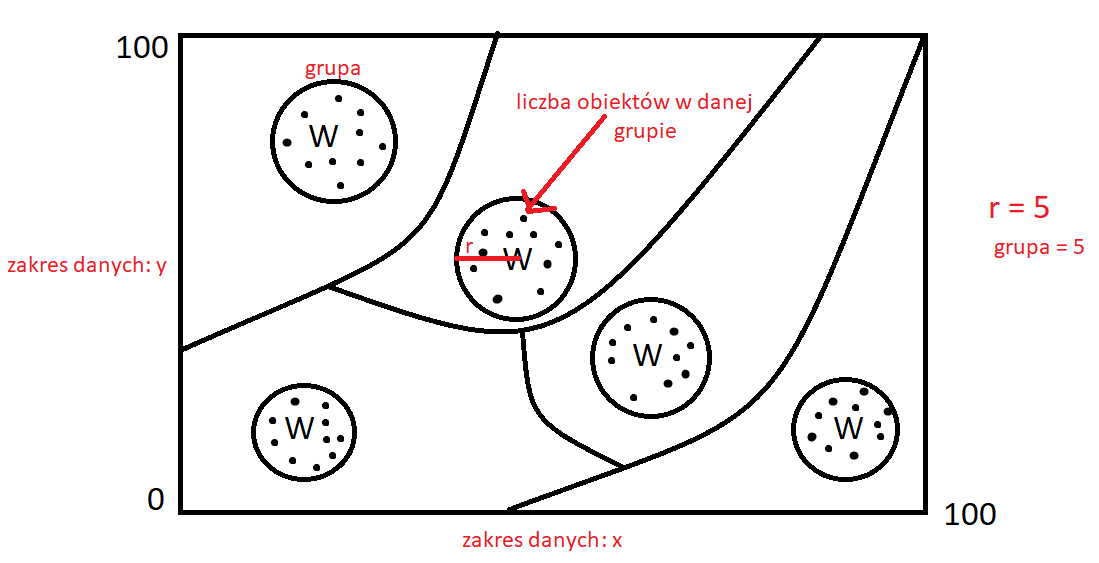
\includegraphics{screeny/WTM_model_example.png}
\end{figure}

UWAGA!!!: Wyświetlanie danych powinno być znormalizowane do zapisu np.
{[}72, 10; \ldots{]}. Każda współrzędna kolejna poprzedzona speratorem
,, ; '\,'

PS: Mieszanie danych podczas uczenia np. w przypadku alfabetu uczenie
(a,b,c,d,\ldots), potem uczenie od (g,h,i,j,\ldots). Różne
możliwości????

    \hypertarget{importowanie-potrzebnych-bibliotek}{%
\subsubsection{Importowanie potrzebnych
bibliotek}\label{importowanie-potrzebnych-bibliotek}}

    \begin{tcolorbox}[breakable, size=fbox, boxrule=1pt, pad at break*=1mm,colback=cellbackground, colframe=cellborder]
\prompt{In}{incolor}{101}{\boxspacing}
\begin{Verbatim}[commandchars=\\\{\}]
\PY{k+kn}{import} \PY{n+nn}{pandas} \PY{k}{as} \PY{n+nn}{pd}
\PY{k+kn}{import} \PY{n+nn}{matplotlib}\PY{n+nn}{.}\PY{n+nn}{pyplot} \PY{k}{as} \PY{n+nn}{plt}
\PY{k+kn}{import} \PY{n+nn}{numpy} \PY{k}{as} \PY{n+nn}{np}
\PY{k+kn}{import} \PY{n+nn}{random}
\PY{k+kn}{import} \PY{n+nn}{math}
\PY{k+kn}{import} \PY{n+nn}{csv}
\end{Verbatim}
\end{tcolorbox}

    \hypertarget{zmienne-potrzebne-do-wygenerowania-danych}{%
\subsubsection{Zmienne potrzebne do wygenerowania
danych}\label{zmienne-potrzebne-do-wygenerowania-danych}}

number\_of\_groups - mienna określająca ilość grup danych

radius - zmienna określająca promień okręgu, który posłużyć ma nam jako
obszar generowanych obiektów danych

number\_of\_object - zmienna mówiąca o ilości obiektów jakie muszą być
wygenerowane w określonej grupie danych

    \begin{tcolorbox}[breakable, size=fbox, boxrule=1pt, pad at break*=1mm,colback=cellbackground, colframe=cellborder]
\prompt{In}{incolor}{102}{\boxspacing}
\begin{Verbatim}[commandchars=\\\{\}]
\PY{n}{number\PYZus{}of\PYZus{}groups} \PY{o}{=} \PY{l+m+mi}{10}    \PY{c+c1}{\PYZsh{}Number of groups in model}
\PY{n}{radius} \PY{o}{=} \PY{l+m+mi}{5}              \PY{c+c1}{\PYZsh{}Circle radius}
\PY{n}{number\PYZus{}of\PYZus{}object} \PY{o}{=} \PY{l+m+mi}{10}   \PY{c+c1}{\PYZsh{}Number of object in each group}
\end{Verbatim}
\end{tcolorbox}

    \hypertarget{proces-generowania-koordynatuxf3w-dla-konkretnych-grup}{%
\subsubsection{Proces generowania koordynatów dla konkretnych
grup}\label{proces-generowania-koordynatuxf3w-dla-konkretnych-grup}}

\begin{itemize}
\tightlist
\item
  za pomocą funkcji ,,zeros'' zawartej w bibliotece numpy generowana
  jest tablica 2D wypełniona zerami, która potem będzie wykorzystana do
  zapisu koordynatów poszczególnych wygenerowanych grup,
\item
  funkcja ,,coordinate\_generator\_group(lst\_groups)`` przekazuje w
  argumencie stworzoną wcześniej tablice 2D wypełnioną zerami. Następnie
  poprzez pętle for przechodzimy po poszczególnych elementach tablicy
  zapisując w niej wygenerowane punkty x i y w odpowiednim zakresie od 0
  do 100. Zapis danych jest poprzez ,,element{[}0{]} \&
  element{[}1{]}'', które zapisują koordynaty w konkretnych miejscach
  podtablicy.
\item
  wykorzystując bibliotekę pandas jesteśmy w stanie zapisać dane x i y w
  dwuwymiarowej strukturze danych, które oznaczone są rzędami i
  kolumnami. Pełni to funkcję przejrzystego wglądu do generowanych
  danych.
\end{itemize}

    \begin{tcolorbox}[breakable, size=fbox, boxrule=1pt, pad at break*=1mm,colback=cellbackground, colframe=cellborder]
\prompt{In}{incolor}{103}{\boxspacing}
\begin{Verbatim}[commandchars=\\\{\}]
\PY{k}{def} \PY{n+nf}{coordinate\PYZus{}generator\PYZus{}group}\PY{p}{(}\PY{n}{temp\PYZus{}lst}\PY{p}{)}\PY{p}{:}
    \PY{k}{for} \PY{n}{element} \PY{o+ow}{in} \PY{n}{temp\PYZus{}lst}\PY{p}{:}
        \PY{n}{temp\PYZus{}x\PYZus{}point} \PY{o}{=} \PY{n}{random}\PY{o}{.}\PY{n}{randint}\PY{p}{(}\PY{l+m+mi}{0}\PY{p}{,}\PY{l+m+mi}{100}\PY{p}{)}    \PY{c+c1}{\PYZsh{}Generate x and y coordinate for specific group}
        \PY{n}{temp\PYZus{}y\PYZus{}point} \PY{o}{=} \PY{n}{random}\PY{o}{.}\PY{n}{randint}\PY{p}{(}\PY{l+m+mi}{0}\PY{p}{,}\PY{l+m+mi}{100}\PY{p}{)}    
        \PY{n}{element}\PY{p}{[}\PY{l+m+mi}{0}\PY{p}{]} \PY{o}{=} \PY{n}{temp\PYZus{}x\PYZus{}point}               \PY{c+c1}{\PYZsh{}Save points in list}
        \PY{n}{element}\PY{p}{[}\PY{l+m+mi}{1}\PY{p}{]} \PY{o}{=} \PY{n}{temp\PYZus{}y\PYZus{}point}
\end{Verbatim}
\end{tcolorbox}

    \begin{tcolorbox}[breakable, size=fbox, boxrule=1pt, pad at break*=1mm,colback=cellbackground, colframe=cellborder]
\prompt{In}{incolor}{104}{\boxspacing}
\begin{Verbatim}[commandchars=\\\{\}]
\PY{n}{lst\PYZus{}groups} \PY{o}{=} \PY{n}{np}\PY{o}{.}\PY{n}{zeros}\PY{p}{(}\PY{p}{(}\PY{n}{number\PYZus{}of\PYZus{}groups}\PY{p}{,}\PY{l+m+mi}{2}\PY{p}{)}\PY{p}{)}    \PY{c+c1}{\PYZsh{}Create a list of groups coordinates}

\PY{n}{coordinate\PYZus{}generator\PYZus{}group}\PY{p}{(}\PY{n}{lst\PYZus{}groups}\PY{p}{)}    \PY{c+c1}{\PYZsh{}Function to generate coordinates for groups}

\PY{n}{groups} \PY{o}{=} \PY{n}{pd}\PY{o}{.}\PY{n}{DataFrame}\PY{p}{(}\PY{n}{lst\PYZus{}groups}\PY{p}{,} \PY{n}{columns} \PY{o}{=}\PY{p}{[}\PY{l+s+s1}{\PYZsq{}}\PY{l+s+s1}{x}\PY{l+s+s1}{\PYZsq{}}\PY{p}{,} \PY{l+s+s1}{\PYZsq{}}\PY{l+s+s1}{y}\PY{l+s+s1}{\PYZsq{}}\PY{p}{]}\PY{p}{)}        \PY{c+c1}{\PYZsh{}Load data groups in DataFrame object}
\PY{n+nb}{print}\PY{p}{(}\PY{n}{groups}\PY{p}{)}
\end{Verbatim}
\end{tcolorbox}

    \begin{Verbatim}[commandchars=\\\{\}]
      x     y
0  26.0  35.0
1  54.0  56.0
2  39.0  19.0
3  52.0  48.0
4  68.0  48.0
5  76.0  84.0
6  64.0  10.0
7  84.0  26.0
8  50.0  15.0
9  21.0  86.0
    \end{Verbatim}

    \hypertarget{proces-generowania-koordynatuxf3w-do-obiektuxf3w-konkretnych-grup-danych}{%
\subsubsection{Proces generowania koordynatów do obiektów konkretnych
grup
danych}\label{proces-generowania-koordynatuxf3w-do-obiektuxf3w-konkretnych-grup-danych}}

\begin{itemize}
\tightlist
\item
  za pomocą wcześniej wspomnianej funkcji ,,zeros'' generowana jest
  tablica 2D wypełniona zerami,
\item
  wspomniana wyżej tablica nadpisywana jest poprzez wywołaną funkcję
  ,,coordinate\_generator\_object(lst\_objects)``. W funkcji na początku
  został stworzony counter, który pomoże podczas identyfkacji danego
  elementu w tablicy temp\_lst, która zawiera
  number\_of\_object*number\_of\_groups elemenetów. Pierwszy człon pętli
  iteruje po elementach tablicy zawierającej koordynaty grup, następny
  człon natomiast będzie generował ilość punktów w grupie zdefiniowanej
  w zmiennej number\_of\_object. Następnie przy pomocy wzorów na ogrąg
  generowane są punkty pod konkretnym kątem w okręgu, który jest grupą
  oraz zapisywane są w zmiennych temp\_x oraz temp\_y. Wygenerowane
  wcześniej koordynaty umieszczane są w konkretnych elementach tablicy
  jaki wskazuje nam zmienna coutner. Na koniec zwracana jest tablica
  wraz z zapisanymi koordynatami.
\item
  rownież z wykorzystaniem biblioteki pandas jesteśmy w sposób
  przejrzysty wyświetlić oraz manipulować danaymi.
\end{itemize}

    \begin{tcolorbox}[breakable, size=fbox, boxrule=1pt, pad at break*=1mm,colback=cellbackground, colframe=cellborder]
\prompt{In}{incolor}{105}{\boxspacing}
\begin{Verbatim}[commandchars=\\\{\}]
\PY{k}{def} \PY{n+nf}{coordinate\PYZus{}generator\PYZus{}object}\PY{p}{(}\PY{n}{temp\PYZus{}lst}\PY{p}{)}\PY{p}{:}
    \PY{n}{counter} \PY{o}{=} \PY{l+m+mi}{0}                                                     \PY{c+c1}{\PYZsh{}counter elements in array temp\PYZus{}lst}
    \PY{k}{for} \PY{n}{elements\PYZus{}lst\PYZus{}groups} \PY{o+ow}{in} \PY{n}{lst\PYZus{}groups}\PY{p}{:}
        \PY{k}{for} \PY{n}{\PYZus{}} \PY{o+ow}{in} \PY{n+nb}{range}\PY{p}{(}\PY{n}{number\PYZus{}of\PYZus{}object}\PY{p}{)}\PY{p}{:}
            \PY{n}{r} \PY{o}{=} \PY{n}{radius} \PY{o}{*} \PY{n}{random}\PY{o}{.}\PY{n}{random}\PY{p}{(}\PY{p}{)}
            \PY{n}{theta} \PY{o}{=} \PY{l+m+mi}{2} \PY{o}{*} \PY{n}{math}\PY{o}{.}\PY{n}{pi} \PY{o}{*}\PY{n}{random}\PY{o}{.}\PY{n}{random}\PY{p}{(}\PY{p}{)}

            \PY{n}{temp\PYZus{}x} \PY{o}{=} \PY{n}{elements\PYZus{}lst\PYZus{}groups}\PY{p}{[}\PY{l+m+mi}{0}\PY{p}{]} \PY{o}{+} \PY{n}{r} \PY{o}{*} \PY{n}{math}\PY{o}{.}\PY{n}{cos}\PY{p}{(}\PY{n}{theta}\PY{p}{)}   \PY{c+c1}{\PYZsh{}Generate x and y coordinate for specific group}
            \PY{n}{temp\PYZus{}y} \PY{o}{=} \PY{n}{elements\PYZus{}lst\PYZus{}groups}\PY{p}{[}\PY{l+m+mi}{1}\PY{p}{]} \PY{o}{+} \PY{n}{r} \PY{o}{*} \PY{n}{math}\PY{o}{.}\PY{n}{sin}\PY{p}{(}\PY{n}{theta}\PY{p}{)}

            \PY{c+c1}{\PYZsh{}print(\PYZsq{}x\PYZsq{}, temp\PYZus{}x, \PYZsq{}y\PYZsq{}, temp\PYZus{}y)}
            \PY{n}{temp\PYZus{}lst}\PY{p}{[}\PY{n}{counter}\PY{p}{]}\PY{p}{[}\PY{l+m+mi}{0}\PY{p}{]} \PY{o}{=} \PY{n}{temp\PYZus{}x}
            \PY{n}{temp\PYZus{}lst}\PY{p}{[}\PY{n}{counter}\PY{p}{]}\PY{p}{[}\PY{l+m+mi}{1}\PY{p}{]} \PY{o}{=} \PY{n}{temp\PYZus{}y}
            \PY{n}{counter}\PY{o}{+}\PY{o}{=}\PY{l+m+mi}{1}
    
    \PY{k}{return} \PY{n}{temp\PYZus{}lst}
\end{Verbatim}
\end{tcolorbox}

    \begin{tcolorbox}[breakable, size=fbox, boxrule=1pt, pad at break*=1mm,colback=cellbackground, colframe=cellborder]
\prompt{In}{incolor}{106}{\boxspacing}
\begin{Verbatim}[commandchars=\\\{\}]
\PY{n}{lst\PYZus{}objects} \PY{o}{=} \PY{n}{np}\PY{o}{.}\PY{n}{zeros}\PY{p}{(}\PY{p}{(}\PY{n}{number\PYZus{}of\PYZus{}object}\PY{o}{*}\PY{n}{number\PYZus{}of\PYZus{}groups}\PY{p}{,} \PY{l+m+mi}{2}\PY{p}{)}\PY{p}{)}     \PY{c+c1}{\PYZsh{}list of object which contain x, y coordinate}

\PY{n}{lst\PYZus{}objects} \PY{o}{=} \PY{n}{coordinate\PYZus{}generator\PYZus{}object}\PY{p}{(}\PY{n}{lst\PYZus{}objects}\PY{p}{)}

\PY{n}{objects} \PY{o}{=} \PY{n}{pd}\PY{o}{.}\PY{n}{DataFrame}\PY{p}{(}\PY{n}{lst\PYZus{}objects}\PY{p}{,} \PY{n}{columns} \PY{o}{=}\PY{p}{[}\PY{l+s+s1}{\PYZsq{}}\PY{l+s+s1}{x}\PY{l+s+s1}{\PYZsq{}}\PY{p}{,} \PY{l+s+s1}{\PYZsq{}}\PY{l+s+s1}{y}\PY{l+s+s1}{\PYZsq{}}\PY{p}{]}\PY{p}{)}        \PY{c+c1}{\PYZsh{}Load data groups in DataFrame object}
\PY{n+nb}{print}\PY{p}{(}\PY{n}{objects}\PY{p}{)}
\end{Verbatim}
\end{tcolorbox}

    \begin{Verbatim}[commandchars=\\\{\}]
            x          y
0   26.467184  32.977646
1   29.231520  34.855235
2   26.097313  34.775430
3   23.889346  36.926630
4   26.030078  38.204176
..        {\ldots}        {\ldots}
95  20.887604  86.107620
96  24.650175  85.141824
97  18.839240  90.286078
98  22.628294  84.851599
99  18.250570  88.257072

[100 rows x 2 columns]
    \end{Verbatim}

    \hypertarget{proces-wyux15bwietlania-wygenerowanych-danych-na-diagramie-z-uux17cyciem-biblioteki-matplotlib}{%
\subsubsection{Proces wyświetlania wygenerowanych danych na diagramie z
użyciem biblioteki
matplotlib}\label{proces-wyux15bwietlania-wygenerowanych-danych-na-diagramie-z-uux17cyciem-biblioteki-matplotlib}}

\begin{itemize}
\tightlist
\item
  Funkcja createCircles(item, radius), do której przekazywane są
  konkretne koordynaty wygenerowanych grup danych oraz promień koła
  wykorzystywane są do określenia środka oraz promienia rysowanego
  okręgu.
\end{itemize}

    \begin{tcolorbox}[breakable, size=fbox, boxrule=1pt, pad at break*=1mm,colback=cellbackground, colframe=cellborder]
\prompt{In}{incolor}{107}{\boxspacing}
\begin{Verbatim}[commandchars=\\\{\}]
\PY{k}{def}  \PY{n+nf}{createCircles}\PY{p}{(}\PY{n}{centre}\PY{p}{,} \PY{n}{radius}\PY{p}{)}\PY{p}{:}
    \PY{k}{return} \PY{n}{plt}\PY{o}{.}\PY{n}{Circle}\PY{p}{(}\PY{p}{(}\PY{n}{centre}\PY{p}{[}\PY{l+m+mi}{0}\PY{p}{]}\PY{p}{,} \PY{n}{centre}\PY{p}{[}\PY{l+m+mi}{1}\PY{p}{]}\PY{p}{)}\PY{p}{,} \PY{n}{radius}\PY{p}{,} \PY{n}{color}\PY{o}{=}\PY{l+s+s1}{\PYZsq{}}\PY{l+s+s1}{b}\PY{l+s+s1}{\PYZsq{}}\PY{p}{,} \PY{n}{fill}\PY{o}{=}\PY{k+kc}{False}\PY{p}{)}
\end{Verbatim}
\end{tcolorbox}

    \begin{tcolorbox}[breakable, size=fbox, boxrule=1pt, pad at break*=1mm,colback=cellbackground, colframe=cellborder]
\prompt{In}{incolor}{108}{\boxspacing}
\begin{Verbatim}[commandchars=\\\{\}]
\PY{c+c1}{\PYZsh{} Creating a new figure }
\PY{n}{fig}\PY{p}{,} \PY{n}{ax} \PY{o}{=} \PY{n}{plt}\PY{o}{.}\PY{n}{subplots}\PY{p}{(}\PY{n}{figsize}\PY{o}{=}\PY{p}{(}\PY{l+m+mi}{10}\PY{p}{,}\PY{l+m+mi}{10}\PY{p}{)}\PY{p}{)}

\PY{c+c1}{\PYZsh{} Numpy array as scatter plot}
\PY{n}{plt}\PY{o}{.}\PY{n}{scatter}\PY{p}{(}\PY{n}{x}\PY{o}{=}\PY{n}{groups}\PY{p}{[}\PY{l+s+s1}{\PYZsq{}}\PY{l+s+s1}{x}\PY{l+s+s1}{\PYZsq{}}\PY{p}{]}\PY{p}{,}\PY{n}{y}\PY{o}{=}\PY{n}{groups}\PY{p}{[}\PY{l+s+s1}{\PYZsq{}}\PY{l+s+s1}{y}\PY{l+s+s1}{\PYZsq{}}\PY{p}{]}\PY{p}{)}
\PY{n}{plt}\PY{o}{.}\PY{n}{scatter}\PY{p}{(}\PY{n}{x}\PY{o}{=}\PY{n}{objects}\PY{p}{[}\PY{l+s+s1}{\PYZsq{}}\PY{l+s+s1}{x}\PY{l+s+s1}{\PYZsq{}}\PY{p}{]}\PY{p}{,}\PY{n}{y}\PY{o}{=}\PY{n}{objects}\PY{p}{[}\PY{l+s+s1}{\PYZsq{}}\PY{l+s+s1}{y}\PY{l+s+s1}{\PYZsq{}}\PY{p}{]}\PY{p}{,} \PY{n}{color}\PY{o}{=} \PY{l+s+s1}{\PYZsq{}}\PY{l+s+s1}{\PYZsh{}f54272}\PY{l+s+s1}{\PYZsq{}}\PY{p}{)}

\PY{n+nb}{print}\PY{p}{(}\PY{n+nb}{len}\PY{p}{(}\PY{n}{lst\PYZus{}groups}\PY{p}{)}\PY{p}{)}

\PY{k}{for} \PY{n}{item} \PY{o+ow}{in} \PY{n}{lst\PYZus{}groups}\PY{p}{:}
    \PY{n}{ax}\PY{o}{.}\PY{n}{add\PYZus{}patch}\PY{p}{(}\PY{n}{createCircles}\PY{p}{(}\PY{n}{item}\PY{p}{,} \PY{n}{radius}\PY{p}{)}\PY{p}{)}

\PY{c+c1}{\PYZsh{} Adding details to the plot}
\PY{n}{plt}\PY{o}{.}\PY{n}{title}\PY{p}{(}\PY{l+s+s1}{\PYZsq{}}\PY{l+s+s1}{Wykres generowanych grup i obiektów}\PY{l+s+s1}{\PYZsq{}}\PY{p}{)}
\PY{n}{plt}\PY{o}{.}\PY{n}{xlabel}\PY{p}{(}\PY{l+s+s1}{\PYZsq{}}\PY{l+s+s1}{x\PYZhy{}axis}\PY{l+s+s1}{\PYZsq{}}\PY{p}{)}
\PY{n}{plt}\PY{o}{.}\PY{n}{ylabel}\PY{p}{(}\PY{l+s+s1}{\PYZsq{}}\PY{l+s+s1}{y\PYZhy{}axis}\PY{l+s+s1}{\PYZsq{}}\PY{p}{)}

\PY{c+c1}{\PYZsh{} Displaying the plot}
\PY{n}{plt}\PY{o}{.}\PY{n}{xlim}\PY{p}{(}\PY{l+m+mi}{0}\PY{p}{,}\PY{l+m+mi}{100}\PY{p}{)}
\PY{n}{plt}\PY{o}{.}\PY{n}{ylim}\PY{p}{(}\PY{l+m+mi}{0}\PY{p}{,}\PY{l+m+mi}{100}\PY{p}{)}
\PY{n}{plt}\PY{o}{.}\PY{n}{grid}\PY{p}{(}\PY{p}{)}
\PY{n}{plt}\PY{o}{.}\PY{n}{show}\PY{p}{(}\PY{p}{)}
\end{Verbatim}
\end{tcolorbox}

    \begin{Verbatim}[commandchars=\\\{\}]
10
    \end{Verbatim}

    \begin{center}
    \adjustimage{max size={0.9\linewidth}{0.9\paperheight}}{WTM_Generator_Finall_Report_files/WTM_Generator_Finall_Report_13_1.png}
    \end{center}
    { \hspace*{\fill} \\}
    
    \hypertarget{zapisywanie-danych-do-pliku-w-celu-wczytania-go-w-programie-kohenen}{%
\subsubsection{Zapisywanie danych do pliku w celu wczytania go w
programie
Kohenen}\label{zapisywanie-danych-do-pliku-w-celu-wczytania-go-w-programie-kohenen}}

Mean quantization error = 9.9677, topographic error = 0.96364

    \begin{tcolorbox}[breakable, size=fbox, boxrule=1pt, pad at break*=1mm,colback=cellbackground, colframe=cellborder]
\prompt{In}{incolor}{109}{\boxspacing}
\begin{Verbatim}[commandchars=\\\{\}]
\PY{k}{with} \PY{n+nb}{open}\PY{p}{(}\PY{l+s+s1}{\PYZsq{}}\PY{l+s+s1}{data\PYZus{}10\PYZus{}temp.dat}\PY{l+s+s1}{\PYZsq{}}\PY{p}{,} \PY{l+s+s1}{\PYZsq{}}\PY{l+s+s1}{w}\PY{l+s+s1}{\PYZsq{}}\PY{p}{,} \PY{n}{newline}\PY{o}{=}\PY{l+s+s1}{\PYZsq{}}\PY{l+s+s1}{\PYZsq{}}\PY{p}{)} \PY{k}{as} \PY{n}{f}\PY{p}{:}
    \PY{n}{csv}\PY{o}{.}\PY{n}{writer}\PY{p}{(}\PY{n}{f}\PY{p}{,} \PY{n}{delimiter}\PY{o}{=}\PY{l+s+s1}{\PYZsq{}}\PY{l+s+s1}{ }\PY{l+s+s1}{\PYZsq{}}\PY{p}{)}\PY{o}{.}\PY{n}{writerows}\PY{p}{(}\PY{n}{lst\PYZus{}groups}\PY{p}{)}
    \PY{n}{csv}\PY{o}{.}\PY{n}{writer}\PY{p}{(}\PY{n}{f}\PY{p}{,} \PY{n}{delimiter}\PY{o}{=}\PY{l+s+s1}{\PYZsq{}}\PY{l+s+s1}{ }\PY{l+s+s1}{\PYZsq{}}\PY{p}{)}\PY{o}{.}\PY{n}{writerows}\PY{p}{(}\PY{n}{lst\PYZus{}objects}\PY{p}{)}
\end{Verbatim}
\end{tcolorbox}

    \hypertarget{teoria-sieci-oraz-analiza-danych-wprowadzonych-w-programie-kohenen}{%
\subsection{Teoria sieci oraz analiza danych wprowadzonych w programie
Kohenen}\label{teoria-sieci-oraz-analiza-danych-wprowadzonych-w-programie-kohenen}}

    \hypertarget{neuronowa-sieux107-kohenena}{%
\subsubsection{Neuronowa sieć
Kohenena}\label{neuronowa-sieux107-kohenena}}

Jest najbardziej znaną i do tego wykorzystywaną siecią samouczącą się,
która realizuje zasadę samoorganizacji (SOM). Jest to także najbardziej
znany przykład sieci konkurencyjnej wykorzystującej koncepcję
sąsiedztwa. W wyniku uczenia powstaje mapa topologiczna, której
aprioryczna interpretacja jest niemożliwa, ponieważ sieć uczy się bez
nauczyciela oraz użytkownik nie jest w stanie kontrolować tego, co się
robi. Natomiast po uczeniu jesteśmy w stanie ustalić jakie poszczególne
rejony mapy majją znaczenie na podstawie analizy danych wejściowych.
Poniższy rysunek przedstawia strukturę sieci Kohonena, gdzie ma on
nakreślić koncepcyjną strukturę schematu, bowiem rzeczywiste sieci
Kohonena cechują się tym, że działają w wielowymiarowych przestrzeniach
danych wejściowych, w związku z czym warstwa wejściowa zawiere bardzo
wiele neuronów (skojarzonych z wieloma sygnałami wejściowymi). Typowa
warstwa topologiczna zawiera również bardzo wiele neuronów, dzięki czemu
sieć po nauczeniu może prezentować bardzo subtelnie rozróżnienia i
klasyfikacje dancyh wejściowych.

\begin{figure}[h]
  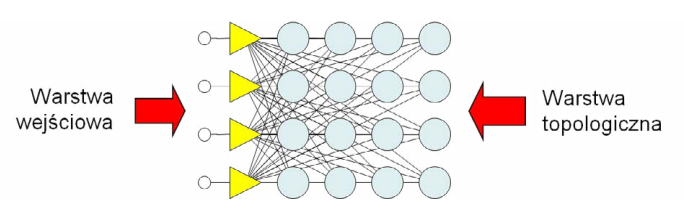
\includegraphics{screeny/Kohonen_network_schema.png}
\end{figure}

\hypertarget{konkurencyjna-sieux107-neuronowa}{%
\subsubsection{Konkurencyjna sieć
neuronowa}\label{konkurencyjna-sieux107-neuronowa}}

W niektórych sieciach neuronowych wśród neuronów warstwy wyjściowej lub
mapy topologicznej wprowadza mechanizm konkurencji, polegający na tym,
że sygnały wyjściowe tych neuronów porównuje się ze sobą. Po podaniu
określonego sygnału wyjściowego do sieci - na jej wyjściu otrzymuje się
sygnały o różnych wartościach pochodzące od różnych neuronów warstwy
wyjściowej lub warstwy topologicznej. Wśród tych sygnałów odnajduje się
ten, który ma największą wartość i ten neuron zostaje wskazany jako
zwycięzca (patrz rysunek). Z faktu, że określony neuron został uznany za
zwycięzcę, wynikają różne konsekwencje. W szczególności w niektórych
sieciach na etapie uczenia zmiany wag dotyczą wyłącznie zwycięzcy oraz
(niekiedy) jego sąsiedztwa. W sieciach klasyfikacyjnych zwycięski neuron
wskazuje poprawną kategoryzację sygnału wejściowego lub poprawne
rozpoznanie obiektu reprezentowanego przez ten sygnał.

\begin{figure}[h!]
  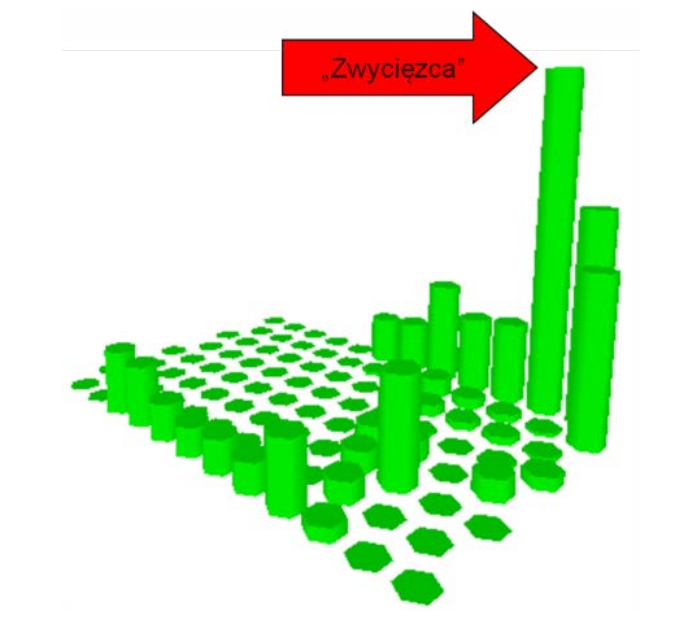
\includegraphics{screeny/concept_winner.png}
\end{figure}

\hypertarget{korekcja-bux142ux119du}{%
\subsubsection{Korekcja błędu}\label{korekcja-bux142ux119du}}

Zmiana wartości parametrów sieci (najczęściej wag) mająca na celu
zmniejszenie błędu popełnianego przez sieć. Ponieważ błąd wyznaczany
jest podczas jednego kroku procesu uczenia, przeto korekta błędu nie
może być zbyt radykalna, bo łatwo jest doprowadzić do sytuacji, w której
zmiana parametrów wynikająca z pokazania jednego przypadku uczącego ze
zbioru uczącego może popsuć wartości parametrów ustalone wcześniej dla
innych przypadków uczących. W praktyce wielkość korekty błędu
determinuje współczynnik uczenia. Przebieg typowej korekty błędu
przedstawia poniższy schemat.

\begin{figure}[h!]
  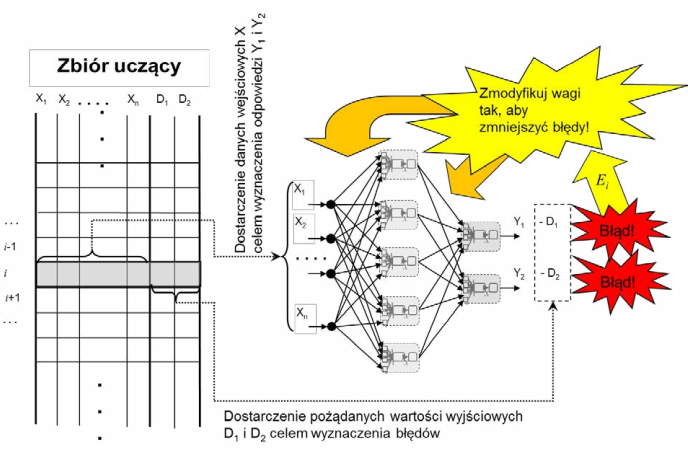
\includegraphics{screeny/corection_fault.png}
\end{figure}

\hypertarget{mapa-topologiczna}{%
\subsubsection{Mapa topologiczna}\label{mapa-topologiczna}}

W sieci Kohonena ta warstwa, na której prezentowany jest wynik działania
sieci, nazywana jest warstwą topologiczną. Neurony należące do tej
warstwy specjalizują się w identyfikowaniu poszczególnych obiektów,
jakie w trakcie procesu samouczenia były sieci prezentowane na jej
wejściu. Każdy neuron warstwy topologicznej ma więc przypisany do siebie
obiekt, którego pojawienie się na wejściu sieci powoduje, że ten właśnie
neuron zostaje zwycięzcą (patrz hasło Konkurencyjna sieć neuronowa).
Rozmieszczenie tych obiektów formuje właśnie mapę topologiczną, pokazaną
symbolicznie na rysunku. Znajomość mapy topologicznej ułatwia
użytkownikowi interpretację i wykorzystanie wyników obliczeń
dostarczanych przez sieć Kohonena.

\begin{figure}[h!]
  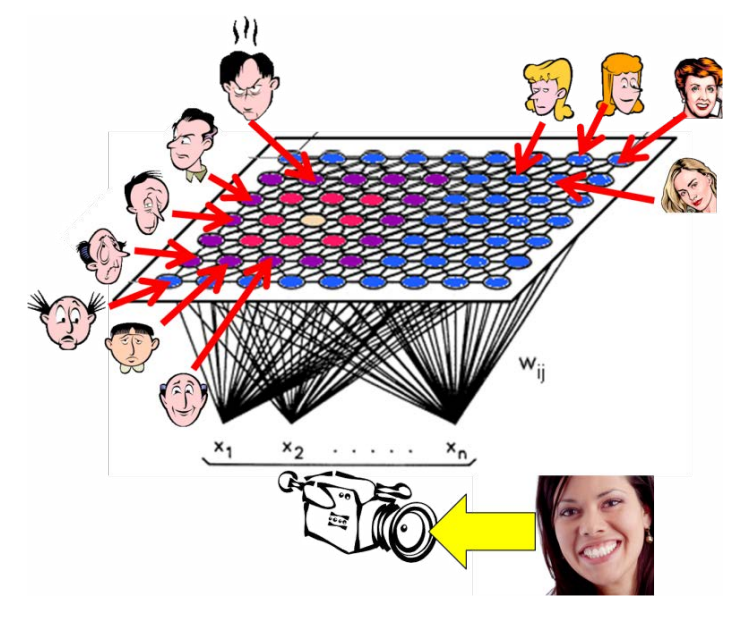
\includegraphics{screeny/topology_map.png}
\end{figure}

\hypertarget{przykux142ady-algorytmuxf3w}{%
\subsubsection{Przykłady algorytmów}\label{przykux142ady-algorytmuxf3w}}

\hypertarget{wta-winner-take-all}{%
\paragraph{WTA (Winner take all)}\label{wta-winner-take-all}}

Algorytm WTA (Winner Takes All) to jeden z podstawowych algorytmów
stosowanych w sieciach neuronowych typu Kohonena, które służą do
grupowania danych wejściowych na podstawie podobieństwa. Algorytm ten
wykorzystuje konkurencyjną regułę uczenia, która pozwala na wyłonienie
zwycięzcy w procesie klasyfikacji.

Algorytm WTA składa się z trzech etapów:

\begin{enumerate}
\def\labelenumi{\arabic{enumi}.}
\tightlist
\item
  Inicjalizacja - losowo inicjuje się położenie neuronów w przestrzeni
  wejściowej i przypisuje im losowe wagi.
\item
  Konkurencja - neuron, który jest najbliżej aktualnie prezentowanego
  wektora wejściowego jest uznawany za zwycięzcę. To właśnie on jest
  aktywowany, a jego wagi są modyfikowane w kierunku wektora
  wejściowego. Wagi pozostałych neuronów pozostają niezmienione. Ten
  etap może być powtarzany wielokrotnie dla różnych wektorów
  wejściowych.
\item
  Stabilizacja - po zakończeniu procesu konkurencji, sieć ulega
  stabilizacji. Wagi neuronów nie są już modyfikowane, a każdy neuron
  jest przypisany do jednej z grup.
\end{enumerate}

Algorytm WTA wykorzystuje zasadę zwycięzcy zabierającego wszystko - to
znaczy, że zwycięzca zabiera całą pulę i jest jedynym neuronem, który
jest aktywowany w trakcie prezentacji danego wektora wejściowego. Dzięki
temu algorytm WTA umożliwia wyłonienie dominującego wzorca wśród danych
wejściowych i grupowanie ich w klastry.

Algorytm WTA znajduje zastosowanie w rozpoznawaniu wzorców, analizie
danych, analizie obrazów oraz klasteryzacji danych. Jego zaletami są
prostota, szybkość i skuteczność. Jednakże, algorytm WTA ma również
pewne wady, takie jak niestabilność w przypadku wystąpienia szumów lub
zmian w danych wejściowych, a także niemożność rozpoznawania złożonych
wzorców.

\hypertarget{wykresy-dla-okreux15blonych-parametruxf3w}{%
\subparagraph{Wykresy dla określonych
parametrów}\label{wykresy-dla-okreux15blonych-parametruxf3w}}

liczba grup = 5 liczba obiektów = 10 liczba epok = 10 wartość początkowa
uczenia = 0.5

\begin{figure}[h]
  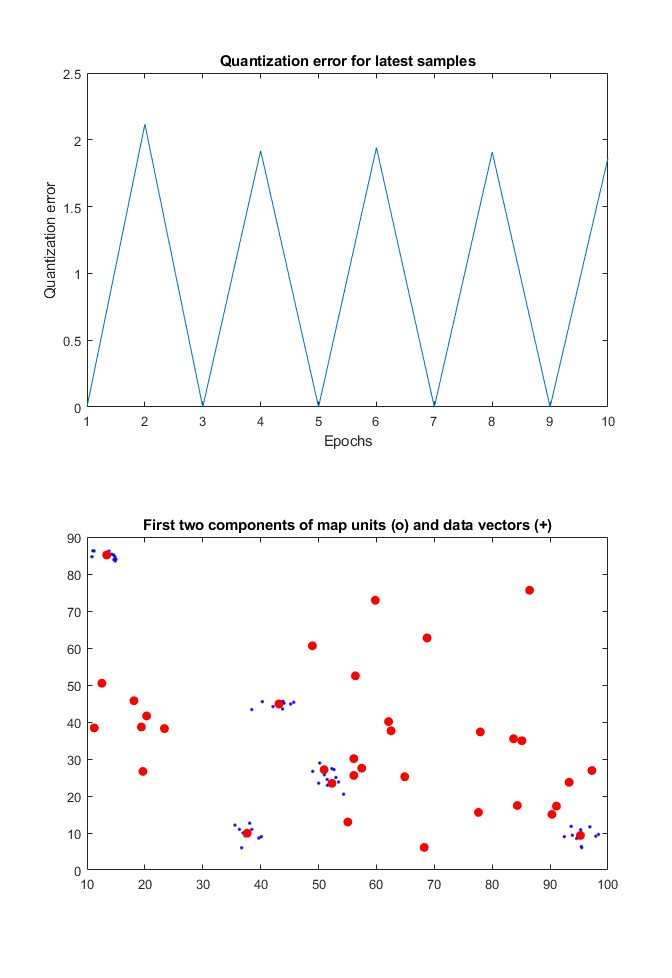
\includegraphics{screeny/WTA/WTA_5_object/WTA_learning_process.jpg}
  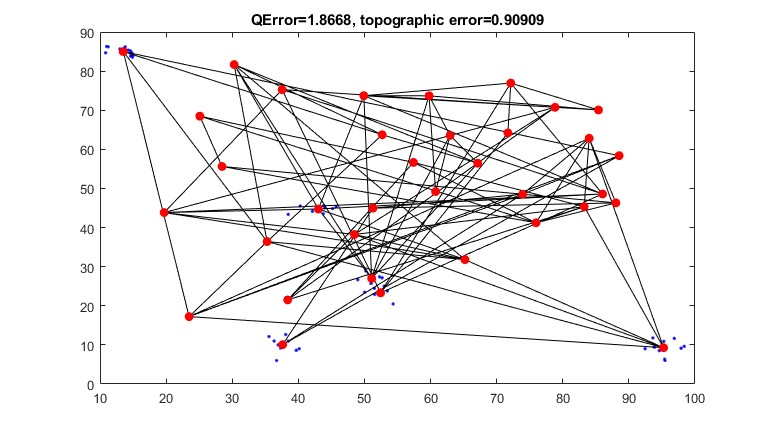
\includegraphics{screeny/WTA/WTA_5_object/WTA_Graph.jpg}
  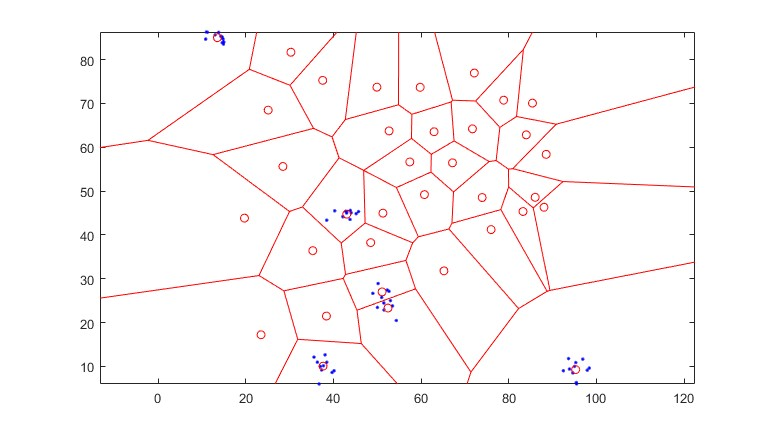
\includegraphics{screeny/WTA/WTA_5_object/WTA_Areas.jpg}
\end{figure}

liczba grup = 10 liczba obiektów = 10 liczba epok = 10 wartość
początkowa uczenia = 0.5

\begin{figure}[h]
  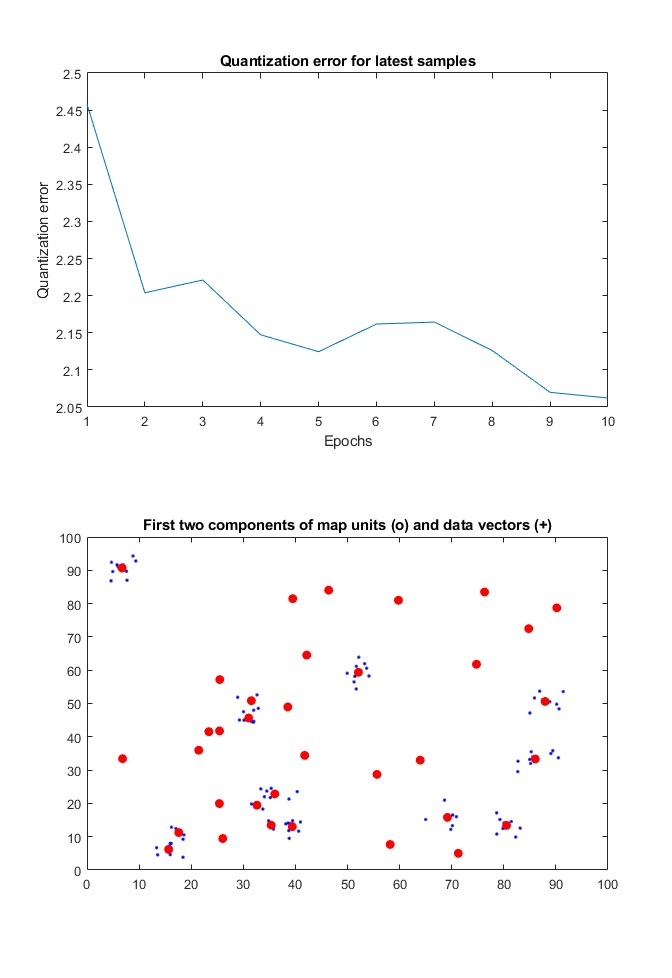
\includegraphics{screeny/WTA/WTA_10_object/WTA_learning_process.jpg}
  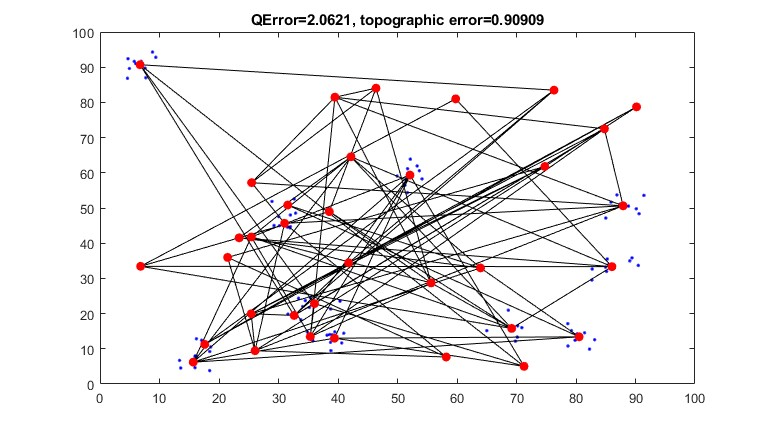
\includegraphics{screeny/WTA/WTA_10_object/WTA_Graph.jpg}
  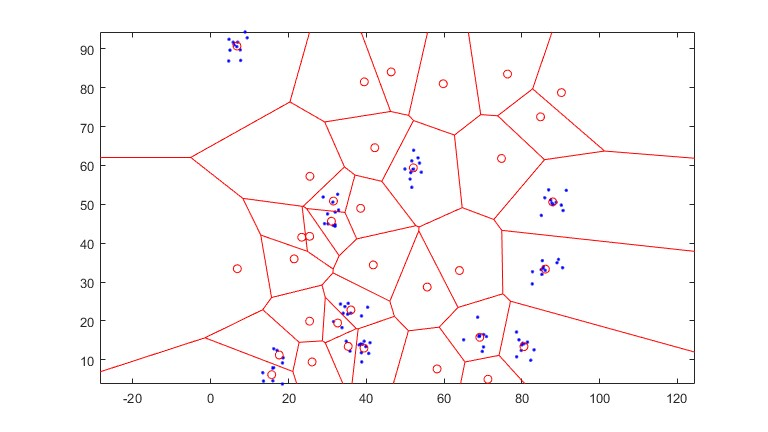
\includegraphics{screeny/WTA/WTA_10_object/WTA_Areas.jpg}
\end{figure}

\hypertarget{cwta-conscience-winner-takes-all}{%
\paragraph{CWTA (Conscience Winner Takes
All)}\label{cwta-conscience-winner-takes-all}}

lgorytm CWTA (Conscience Winner Takes All) to modyfikacja standardowego
algorytmu Winner-Takes-All (WTA), stosowanego w sieciach neuronowych
typu Kohonena. WTA wybiera zwycięzcę na podstawie minimalnej odległości
między wektorem wejściowym a neuronami SOM. WTA nie uwzględnia jednak
dodatkowej wiedzy o stanie sieci, co może prowadzić do niedopasowania
zwycięzcy.

Algorytm CWTA wprowadza pojęcie ``sumy sumień'' dla każdego neuronu,
która odzwierciedla aktywność neuronu na przestrzeni czasu. Im częściej
neuron jest aktywny, tym wyższa jest jego suma sumień. Dzięki temu, że
CWTA uwzględnia historię aktywności neuronów, pozwala na wybór bardziej
stabilnego zwycięzcy, który jest w stanie lepiej odzwierciedlić
strukturę wejściową.

Algorytm CWTA składa się z dwóch faz:

\begin{enumerate}
\def\labelenumi{\arabic{enumi}.}
\tightlist
\item
  Faza konkurencji - każdy neuron SOM jest aktywowany przez wektor
  wejściowy, a następnie suma sumień każdego neuronu jest zwiększana o
  wartość procentową.
\item
  Faza selekcji zwycięzcy - neuron z najniższą wartością sumy sumień
  jest uznawany za zwycięzcę i jest aktualizowany.
\end{enumerate}

Algorytm CWTA pozwala na uniknięcie efektu ``histerii'' sieci, gdzie
zwycięzca stale wygrywa, a inne neurony są wykluczone. Dzięki
uwzględnieniu historii aktywności, algorytm CWTA może przeciwdziałać
temu efektowi, wybierając bardziej stabilnych zwycięzców i zapewniając
bardziej równomierne rozmieszczenie neuronów SOM w przestrzeni
wejściowej.

Algorytm CWTA znajduje zastosowanie w rozpoznawaniu wzorców,
klasyfikacji obrazów i analizie danych, gdzie ważna jest stabilność
wyboru zwycięzcy i równomierność rozkładu neuronów SOM w przestrzeni
wejściowej.

\hypertarget{wykresy-dla-okreux15blonych-parametruxf3w-1}{%
\subparagraph{Wykresy dla określonych
parametrów}\label{wykresy-dla-okreux15blonych-parametruxf3w-1}}

liczba grup = 5 liczba obiektów = 10 liczba epok = 10 wartość początkowa
uczenia = 0.5

\begin{figure}[h!]
  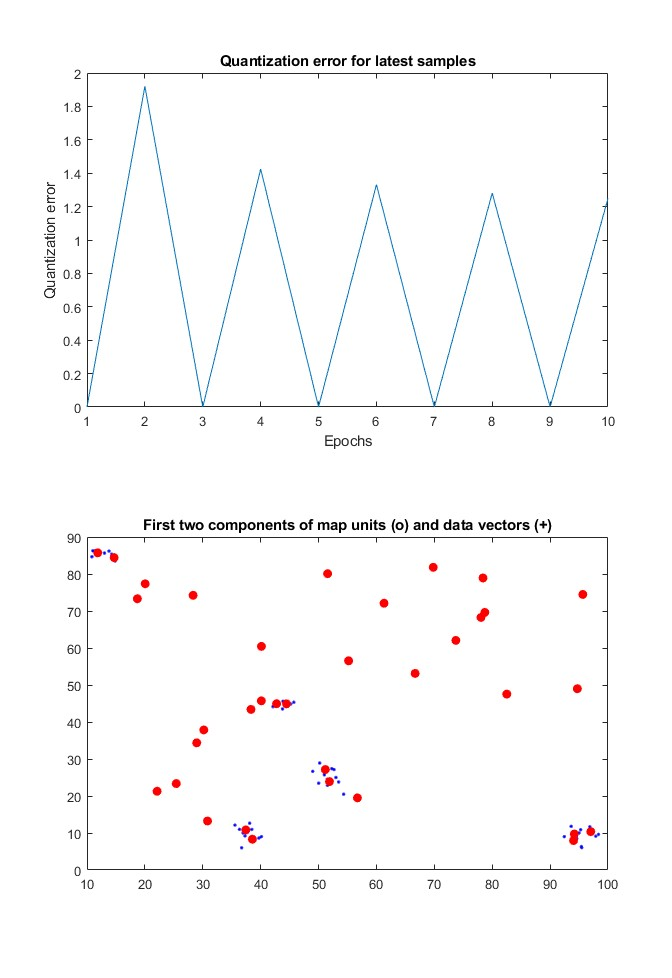
\includegraphics{screeny/CWTA/CWTA_5_groups/CWTA_learning_process.jpg}
  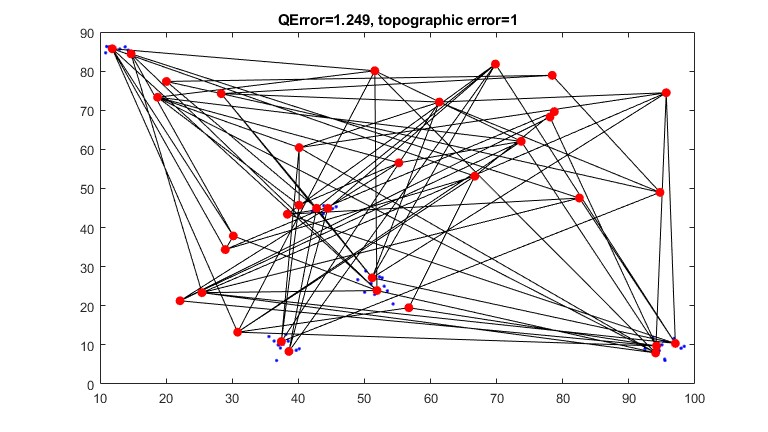
\includegraphics{screeny/CWTA/CWTA_5_groups/CWTA_Graph.jpg}
  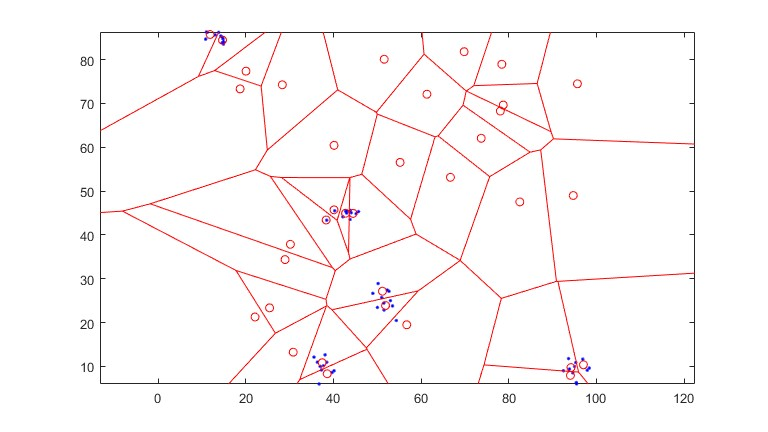
\includegraphics{screeny/CWTA/CWTA_5_groups/CWTA_Areas.jpg}
\end{figure}

liczba grup = 10 liczba obiektów = 10 liczba epok = 10 wartość
początkowa uczenia = 0.5

\begin{figure}[h!]
  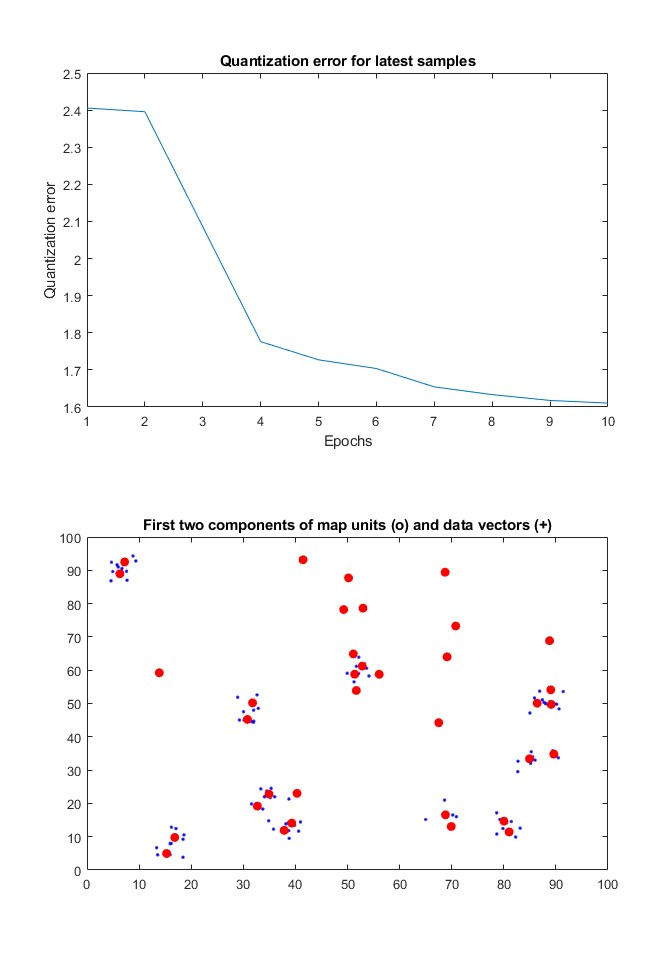
\includegraphics{screeny/CWTA/CWTA_10_groups/CWTA_learning_process.jpg}
  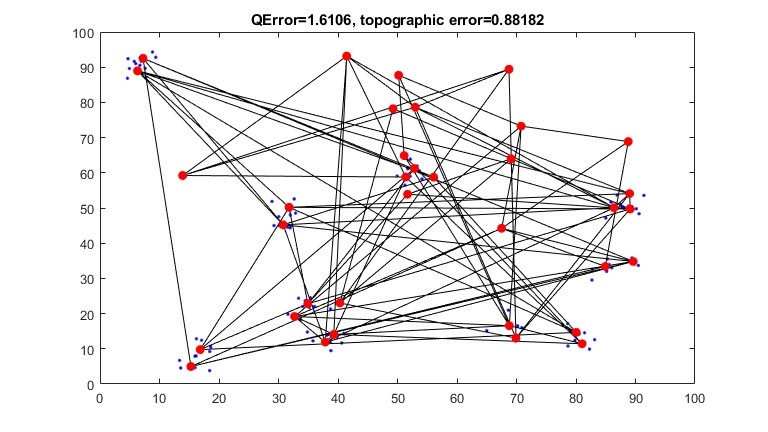
\includegraphics{screeny/CWTA/CWTA_10_groups/CWTA_Graph.jpg}
  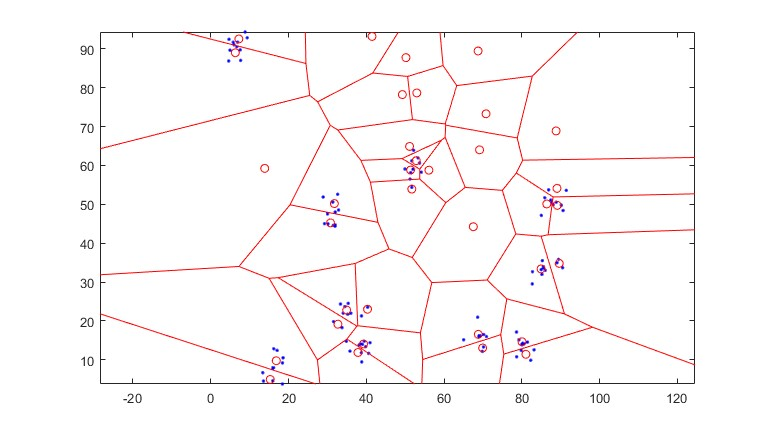
\includegraphics{screeny/CWTA/CWTA_10_groups/CWTA_Areas.jpg}
\end{figure}

\hypertarget{wtm-batch-winner-takes-most-batch}{%
\paragraph{WTM batch (Winner Takes Most
Batch)}\label{wtm-batch-winner-takes-most-batch}}

Algorytm WTM Batch (Winner Takes Most Batch) jest stosowany w sieciach
neuronowych typu Kohonena, które służą do grupowania danych wejściowych
na podstawie podobieństwa. Algorytm ten składa się z dwóch faz:
inicjalizacji i konkurencji.

\begin{enumerate}
\def\labelenumi{\arabic{enumi}.}
\item
  Inicjalizacja: W fazie inicjalizacji losowo wybierane są wagi dla
  neuronów SOM (Self-Organizing Map). Wagi te są przypisywane
  początkowemu rozkładowi w przestrzeni wejściowej.
\item
  Konkurencja: W fazie konkurencji dla każdego wejścia wyznaczany jest
  neuron z najbliższą wagą, zwany zwycięzcą. Następnie wagi są
  aktualizowane, tak aby zwycięzca miał jeszcze bliższe wartości do
  wejścia, a sąsiednie neurony do zwycięzcy również są aktualizowane,
  ale w mniejszym stopniu.
\end{enumerate}

Algorytm WTM Batch wykorzystuje strategię zwycięzca-bierze-więcej
(winner-takes-most), co oznacza, że wybrany neuron otrzymuje większą
aktualizację swoich wag, a sąsiednie neurony są aktualizowane w
mniejszym stopniu. Dzięki temu algorytm może szybciej osiągać
stabilizację i lepiej radzić sobie z dużymi zbiorami danych.

Algorytm WTM Batch jest stosowany w przetwarzaniu obrazów i dźwięku,
gdzie sieci Kohonena służą do grupowania pikseli lub cech dźwiękowych w
zbiory o podobnych właściwościach.

\hypertarget{wykresy-dla-okreux15blonych-parametruxf3w-2}{%
\subparagraph{Wykresy dla określonych
parametrów}\label{wykresy-dla-okreux15blonych-parametruxf3w-2}}

liczba grup = 5 liczba obiektów = 10 liczba epok = 10 wartość początkowa
uczenia = 0.2 promień początkowy = 3

\begin{figure}[h!]
  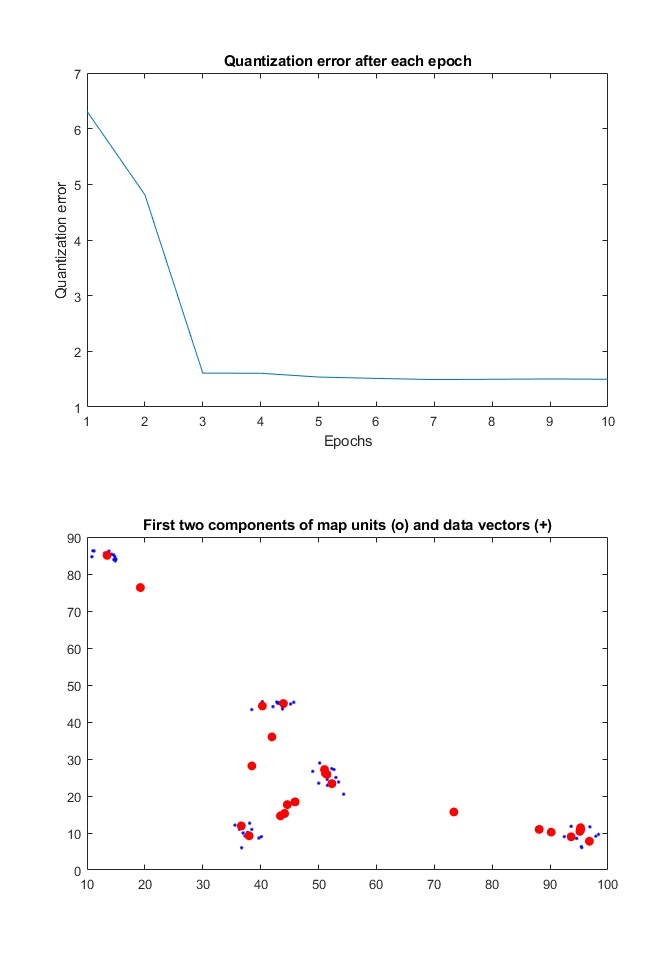
\includegraphics{screeny/WTM_batch/WTM_batch_5_groups/WTM_batch_learning_process.jpg}
  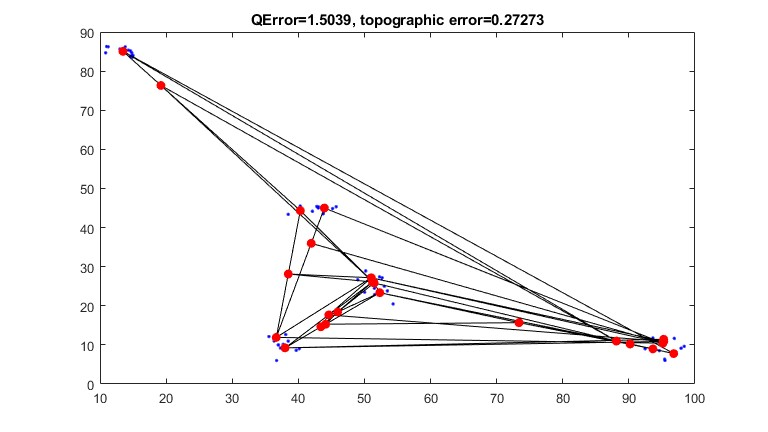
\includegraphics{screeny/WTM_batch/WTM_batch_5_groups/WTM_batch_Graph.jpg}
  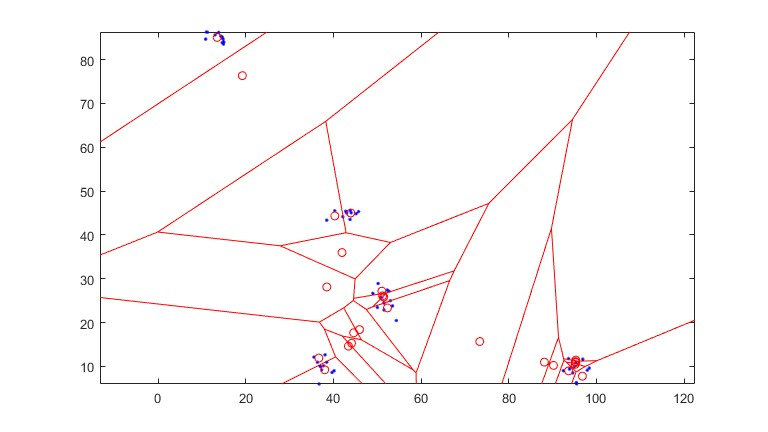
\includegraphics{screeny/WTM_batch/WTM_batch_5_groups/WTM_batch_Areas.jpg}
\end{figure}

liczba grup = 10 liczba obiektów = 10 liczba epok = 10 wartość
początkowa uczenia = 0.2 promień początkowy = 3

\begin{figure}[h!]
  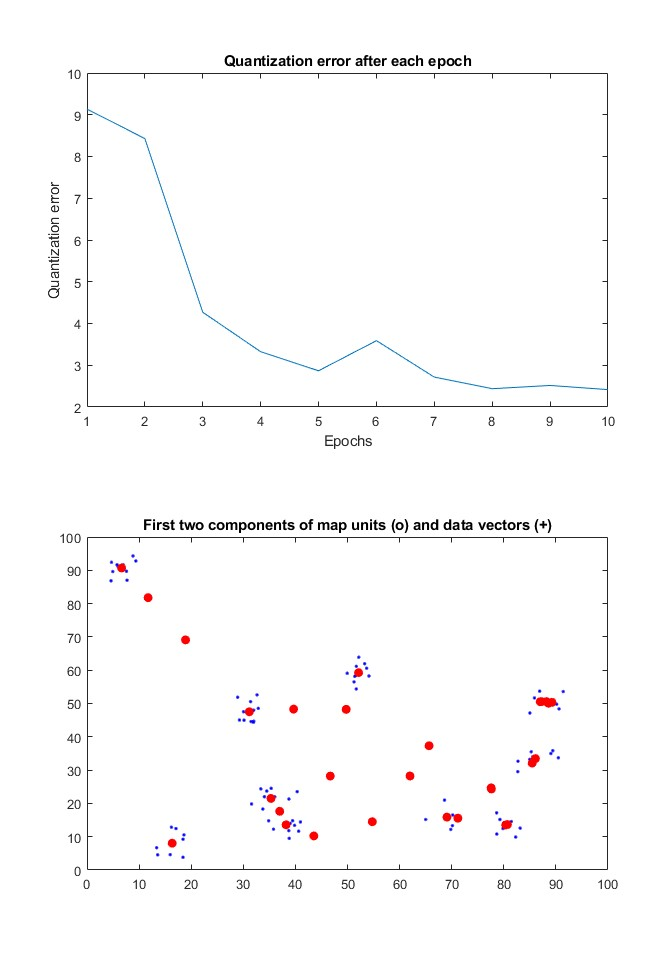
\includegraphics{screeny/WTM_batch/WTM_batch_10_groups/WTM_batch_learning_process.jpg}
  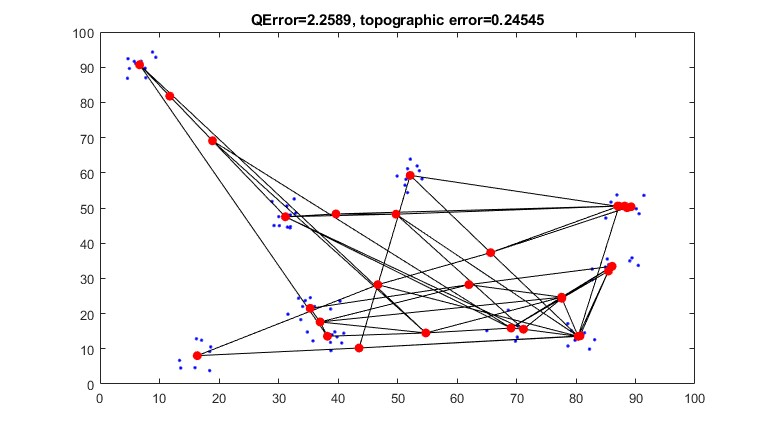
\includegraphics{screeny/WTM_batch/WTM_batch_10_groups/WTM_batch_Graph.jpg}
  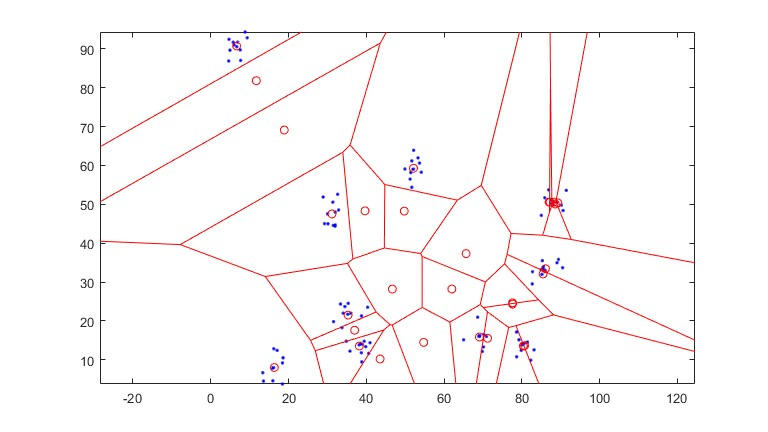
\includegraphics{screeny/WTM_batch/WTM_batch_10_groups/WTM_batch_Areas.jpg}
\end{figure}

\hypertarget{wtm-seq}{%
\paragraph{WTM seq}\label{wtm-seq}}

Algorytm WTM Seq (Winner Takes Most Sequence) jest rozszerzeniem
algorytmu WTM Batch, również stosowanym w sieciach neuronowych typu
Kohonena. W odróżnieniu od WTM Batch, WTM Seq uwzględnia sekwencje
danych wejściowych i ma zastosowanie w analizie sekwencji tekstu.

Algorytm WTM Seq składa się z trzech faz:

\begin{enumerate}
\def\labelenumi{\arabic{enumi}.}
\tightlist
\item
  Inicjalizacji - losowo wybierane są wagi dla neuronów SOM.
\item
  Konkurencji - dla każdej sekwencji wyznaczany jest neuron z najbliższą
  wagą, zwany zwycięzcą. Wagi są aktualizowane, aby zwycięzca miał
  jeszcze bliższe wartości do sekwencji, a sąsiednie neurony do
  zwycięzcy również są aktualizowane, ale w mniejszym stopniu.
\item
  Adaptacji - po każdej iteracji uczącej wagi są aktualizowane w sposób
  specyficzny dla sekwencji. Zamiast aktualizować wagi neuronów tylko na
  podstawie jednej sekwencji, algorytm WTM Seq wykorzystuje wagę
  neuronu, która zależy od sumy wag zwycięzców dla każdej sekwencji w
  ciągu uczącym. To znaczy, że sekwencje występujące częściej wpłyną na
  aktualizację wag w sposób bardziej znaczący.
\end{enumerate}

Algorytm WTM Seq jest stosowany w analizie sekwencji tekstu, na przykład
do grupowania dokumentów na podstawie podobieństwa. Może być również
stosowany w innych dziedzinach, gdzie występują sekwencje danych
wejściowych, takich jak sekwencje DNA lub sygnały czasowe.

\hypertarget{wykresy-dla-okreux15blonych-parametruxf3w-3}{%
\subparagraph{Wykresy dla określonych
parametrów}\label{wykresy-dla-okreux15blonych-parametruxf3w-3}}

liczba grup = 5 liczba obiektów = 10 liczba epok = 10 wartość początkowa
uczenia = 0.05 promień początkowy = 4

\begin{figure}[h!]
  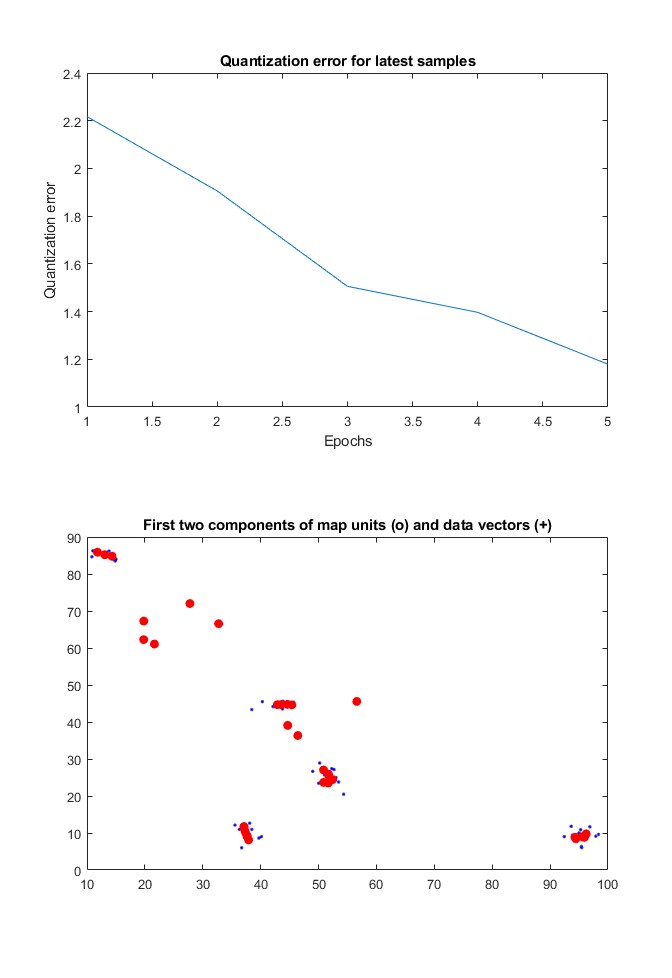
\includegraphics{screeny/WTM_seq/WTM_seq_5_groups/WTM_seq_learning_process.jpg}
  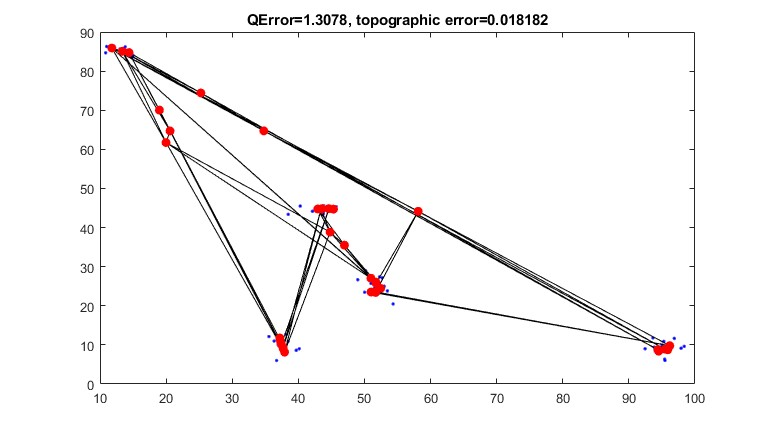
\includegraphics{screeny/WTM_seq/WTM_seq_5_groups/WTM_seq_Graph.jpg}
  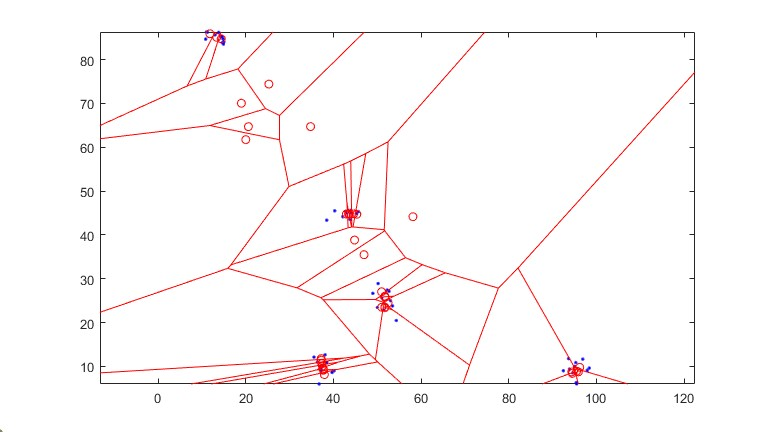
\includegraphics{screeny/WTM_seq/WTM_seq_5_groups/WTM_seq_Areas.jpg}
\end{figure}

liczba grup = 10 liczba obiektów = 10 liczba epok = 10 wartość
początkowa uczenia = 0.05 promień początkowy = 4

\begin{figure}[h!]
  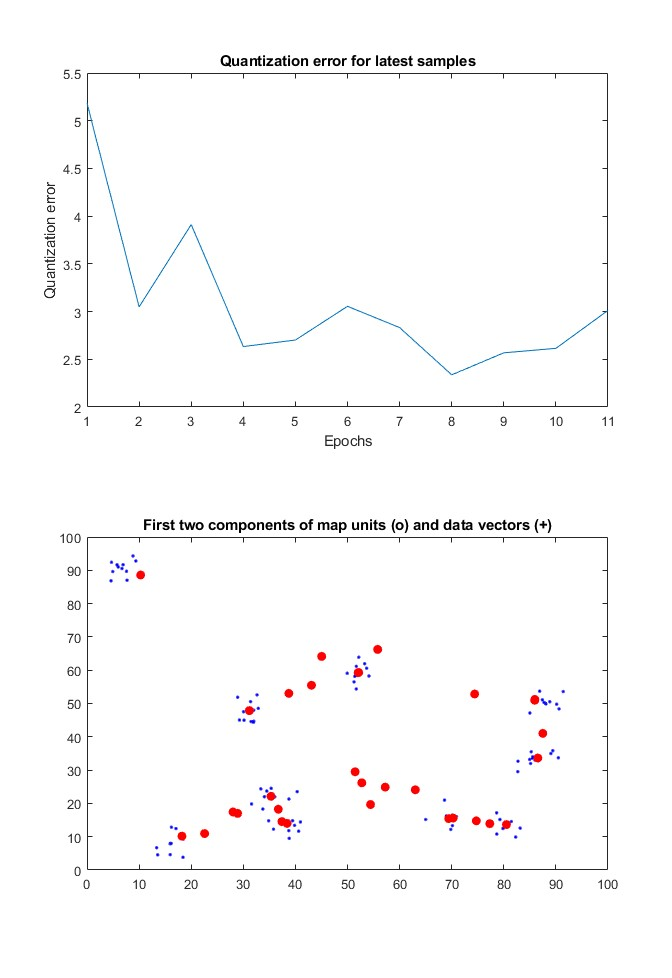
\includegraphics{screeny/WTM_seq/WTM_seq_10_groups/WTM_seq_learning_process.jpg}
  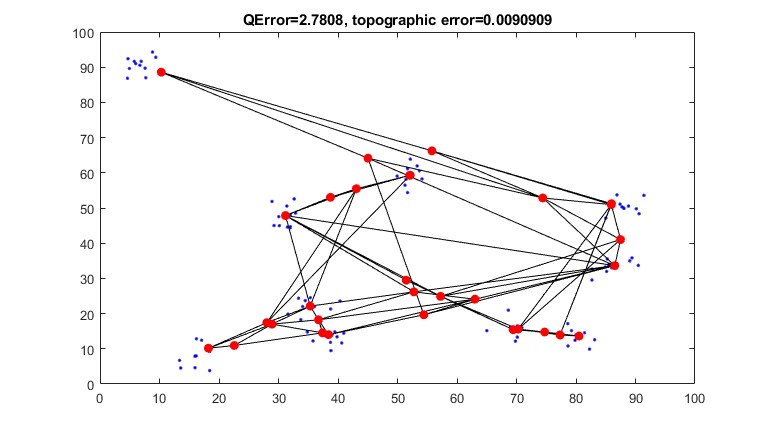
\includegraphics{screeny/WTM_seq/WTM_seq_10_groups/WTM_seq_Graph.jpg}
  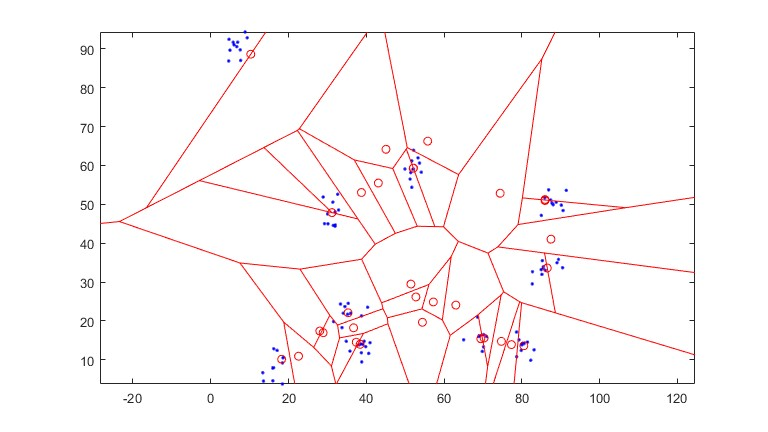
\includegraphics{screeny/WTM_seq/WTM_seq_10_groups/WTM_seq_Areas.jpg}
\end{figure}

\hypertarget{neutral-gas}{%
\paragraph{Neutral gas}\label{neutral-gas}}

Algorytm Neural Gas (NG) jest jednym z algorytmów stosowanych w sieciach
neuronowych typu Kohonena, które służą do grupowania danych wejściowych
na podstawie podobieństwa. Algorytm ten jest rozszerzeniem algorytmu
Kohonena i wykorzystuje podobne założenia co WTM (Winner-Takes-Most).

Algorytm NG składa się z trzech etapów:

\begin{enumerate}
\def\labelenumi{\arabic{enumi}.}
\tightlist
\item
  Inicjalizacja - losowo inicjuje się położenie neuronów w przestrzeni
  wejściowej i przypisuje im losowe wagi.
\item
  Adaptacja - neuron, który jest najbliżej aktualnie prezentowanego
  wektora wejściowego jest uaktualniany poprzez zmianę swojej pozycji
  oraz wagi. Sąsiedzi tego neuronu również są uaktualniani, ale w
  mniejszym stopniu. Proces ten jest powtarzany wielokrotnie aż do
  osiągnięcia stabilizacji.
\item
  Redukcja - usuwanie neuronów, które są mniej aktywne i nie
  przyczyniają się do zdefiniowania skutecznych klastrów.
\end{enumerate}

Algorytm NG różni się od standardowej sieci Kohonena tym, że bada on
dystrybucję punktów w przestrzeni wejściowej, a nie odległość
euklidesową między neuronami. W wyniku tego algorytm NG umożliwia
bardziej równomierne rozmieszczenie neuronów w przestrzeni wejściowej
oraz lepsze przewidywanie topologii rozkładu klastrów.

Algorytm Neural Gas znajduje zastosowanie w rozpoznawaniu wzorców,
analizie danych, analizie obrazów oraz klasteryzacji danych.

\hypertarget{wykresy-dla-okreux15blonych-parametruxf3w-4}{%
\subparagraph{Wykresy dla określonych
parametrów}\label{wykresy-dla-okreux15blonych-parametruxf3w-4}}

liczba grup = 5 liczba obiektów = 10 liczba epok = 10 wartość początkowa
uczenia = 0.5 lambda początkowa = 18

\begin{figure}[h!]
  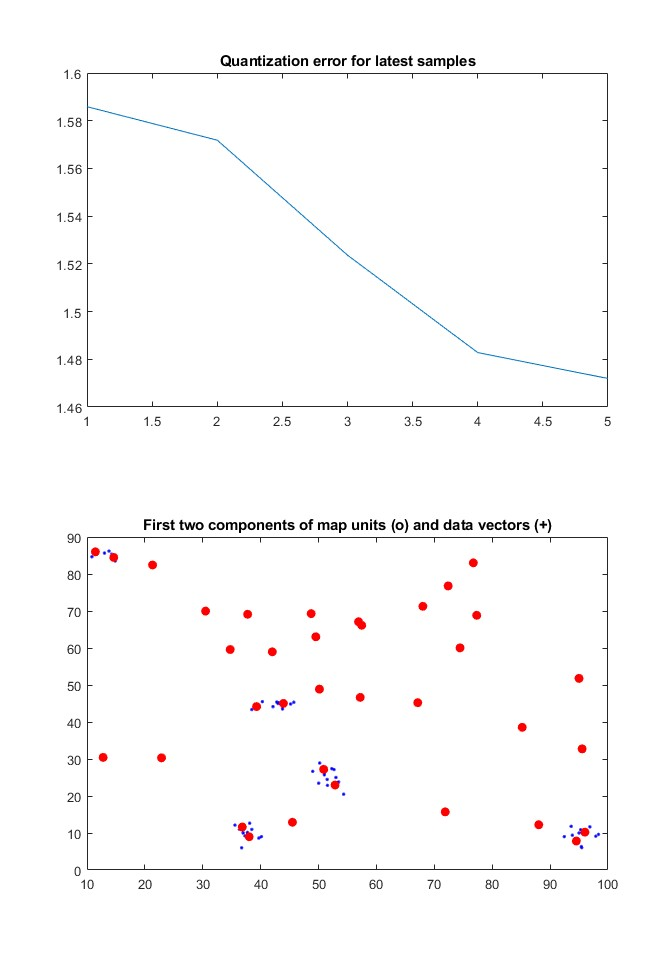
\includegraphics{screeny/NeuralGas/Neural_gasp_5_groups/Neural_gasp_learning_process.jpg}
  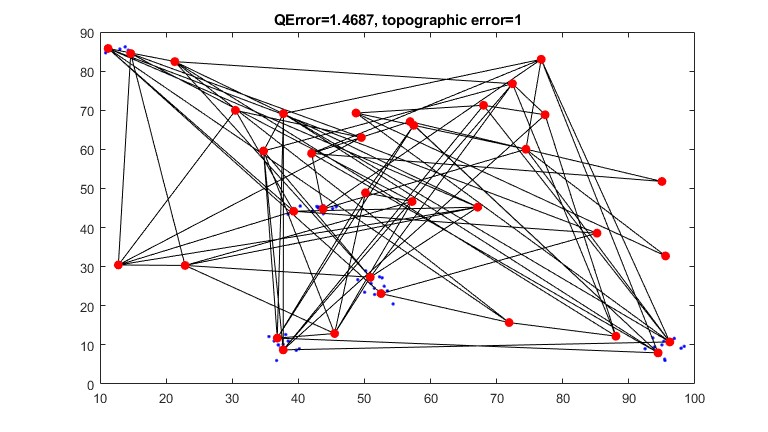
\includegraphics{screeny/NeuralGas/Neural_gasp_5_groups/Neural_gasp_Graph.jpg}
  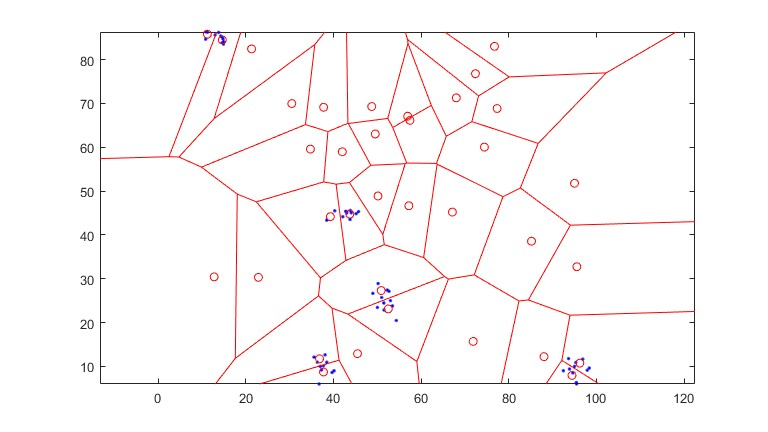
\includegraphics{screeny/NeuralGas/Neural_gasp_5_groups/Neural_gasp_Areas.jpg}
\end{figure}

liczba grup = 10 liczba obiektów = 10 liczba epok = 10 wartość
początkowa uczenia = 0.5 lambda początkowa = 18

\begin{figure}[h!]
  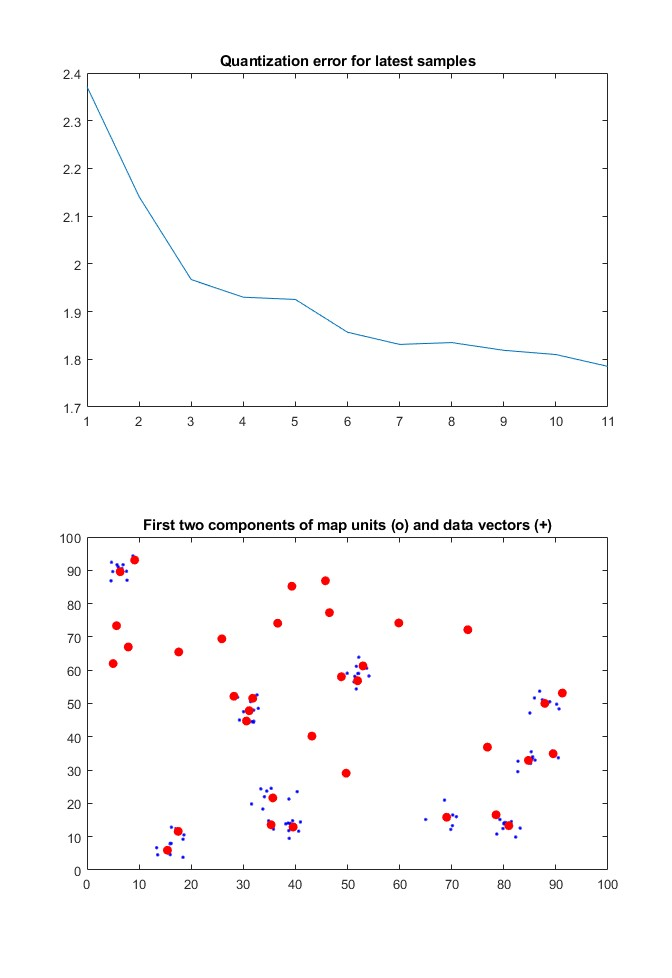
\includegraphics{screeny/NeuralGas/Neural_gasp_10_groups/Neural_gasp_learning_process.jpg}
  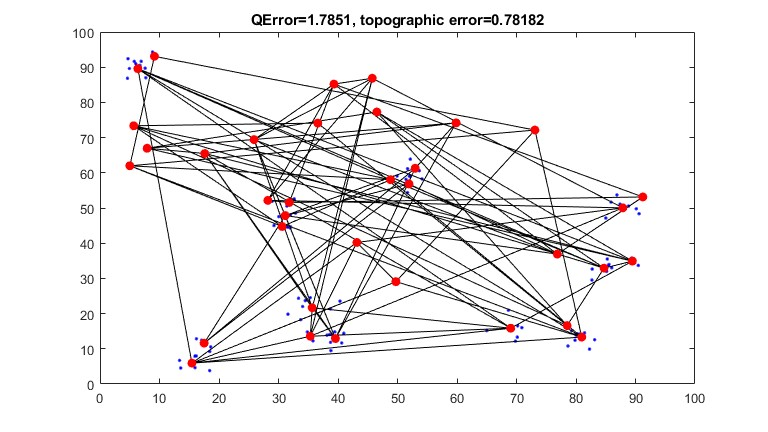
\includegraphics{screeny/NeuralGas/Neural_gasp_10_groups/Neural_gasp_Graph.jpg}
  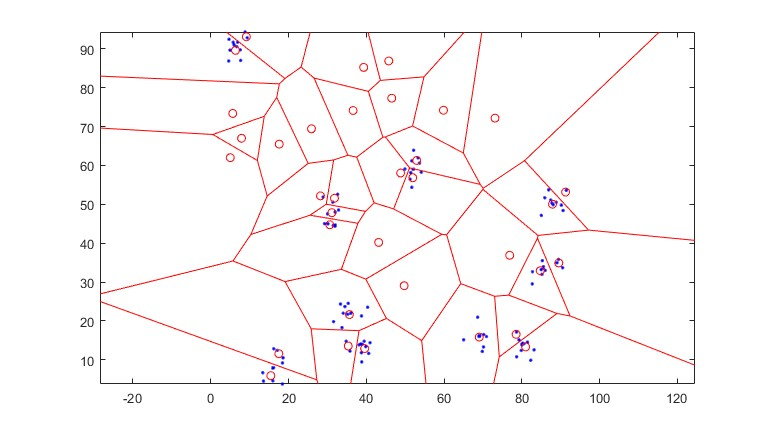
\includegraphics{screeny/NeuralGas/Neural_gasp_10_groups/Neural_gasp_Areas.jpg}
\end{figure}

\hypertarget{podsumowanie-oraz-wnioski}{%
\subsubsection{Podsumowanie oraz
wnioski}\label{podsumowanie-oraz-wnioski}}

Podsumowując, algorytmy w sieciach neuronowych typu Kohonena służą do
grupowania danych wejściowych w klastry. Wyróżniamy kilka algorytmów,
takich jak WTA, CWTA, Neural Gas oraz WTM batch i WTM seq, które różnią
się między sobą sposobem wyłaniania zwycięzców i modyfikacji wag
neuronów.

Niezbędnym elementem w sieciach Kohonena jest proces kwantyzacji, czyli
przypisywania wektorów wejściowych do najbliższego neuronu. Jednakże,
ten proces może wprowadzić błąd kwantyzacji, co z kolei może prowadzić
do destabilizacji sieci i utraty jakości grupowania.

W algorytmie WTA, błąd kwantyzacji jest duży wynika z faktu, że
wyłoniony zwycięzca reprezentuje tylko jeden klaster, co może prowadzić
do nieprawidłowego grupowania danych wejściowych, szczególnie w
przypadku wystąpienia szumów lub zmian w danych.

W algorytmie CWTA, błąd kwantyzacji jest mniejszy, ponieważ mechanizm
sumy sumień umożliwia zapobieganie powstawaniu klastrów o niskiej
jakości. Niemniej jednak, nadal istnieje ryzyko nieprawidłowego
grupowania danych wejściowych.

W algorytmie Neural Gas, błąd kwantyzacji jest redukowany poprzez
rozproszenie neuronów w przestrzeni wejściowej, co umożliwia
dokładniejsze odwzorowanie danych i wyłonienie mniejszych, bardziej
precyzyjnych klastrów.

W algorytmach WTM batch oraz WTM seq, błąd kwantyzacji jest mniejszy niż
w algorytmie WTA, ponieważ umożliwiają wyłonienie kilku zwycięzców dla
danego wektora wejściowego. To pozwala na zredukowanie ryzyka
nieprawidłowego grupowania danych i zwiększenie stabilności sieci.

Wnioskiem z powyższego jest to, że błąd kwantyzacji jest kluczowym
problemem w sieciach neuronowych typu Kohonena, a wybór odpowiedniego
algorytmu zależy od specyfiki problemu, rodzaju danych wejściowych oraz
wymagań dotyczących stabilności i jakości grupowania.


    % Add a bibliography block to the postdoc
    
    
    
\end{document}
